\documentclass[a4paper]{amsbook}
\usepackage[
    backend=biber,
    style=ieee,
    sorting=ynt
]{biblatex}
\addbibresource{../references/fundamentals.bib}
\addbibresource{../references/imaging.bib}
\usepackage{graphicx,caption,subcaption,amsmath,amssymb,svg,hyperref,siunitx,trfsigns,listings,float}
\sisetup{exponent-product = \cdot}
\DeclareSIUnit{\belrelative}{Br}
\DeclareSIUnit{\dBr}{\deci\belrelative}

\definecolor{codegreen}{rgb}{0.2,0.6,0}
\definecolor{codegray}{rgb}{0.5,0.5,0.5}
\definecolor{codered}{rgb}{0.7,0.2,0.0}
\definecolor{codeteal}{rgb}{0.0,0.4,0.82}
\definecolor{backcolour}{rgb}{0.95,0.95,0.95}

\lstdefinestyle{mystyle}{
    backgroundcolor=\color{backcolour},
    commentstyle=\color{codegreen},
    keywordstyle=\color{codeteal},
    numberstyle=\tiny\color{codegray},
    stringstyle=\color{codered},
    basicstyle=\ttfamily\footnotesize,
    breakatwhitespace=false,  
    breaklines=true,
    captionpos=b,
    keepspaces=true,
    numbers=left,
    numbersep=5pt,
    showspaces=false,
    showstringspaces=false,
    showtabs=false,
    tabsize=2
} 
\numberwithin{figure}{chapter} 
\setlength{\headheight}{12.0pt}

\begin{document}
\begin{titlepage}
    \begin{center}
        \vspace*{1cm}

        \huge
        \textbf{Calibration and Image Reconstruction Techniques
            for FMCW MIMO Radars with Consideration of Antenna Radiation Patterns}
        \vspace{0.5cm}

        \large
        Kalibrations- und Bildrekonstruktionsverfahren für FMCW-MIMO-Radare unter Berücksichtigung der Antennenabstrahlungscharakteristik
        \vspace{1.5cm}

        \textbf{Daniel Gotzens}

        \vfill

        \normalsize
        Masterarbeit vorgelegt dem \\

        \vspace{0.8cm}

        
\includegraphics[height=18pt]{../figures/IHF-Logo_platzhalter.png}

        Lehrstuhl für Radarsystemtechnik \\
        Institut für Hochfrequenztechnik \\
        RWTH Aachen University\\
        \today

        \vspace{1cm}
        In Kooperation mit \\

        
\includegraphics[height=18pt]{../figures/indurad-logo.png}

        indurad GmbH
        Aachen

    \end{center}
\end{titlepage}

\begin{abstract}
    Increased image quality can be achieved by implementing backprojection on a millimeter-wave TDM FMCW MIMO Radar.
    In this thesis, a backprojection-based imaging algorithm is proposed and implemented for a radar sensor.
    This radar sensor's functionality is tested, the sensor is calibrated,
    and then the algorithm is compared to the current FFT-based algorithm as well as MUSIC.
    It is found that near-field accuracy of the image generated with backprojection and MUSIC is increased,
    and that real-time capability can only be guaranteed for backprojection and the current FFT-based approach.
\end{abstract}

\setcounter{tocdepth}{2}
\tableofcontents

\chapter{Introduction}

Radar technology has undergone significant advancements over the decades,
revolutionizing various fields including aerospace, defense, automotive, and healthcare.
Its fundamental principle of using electromagnetic waves to detect the presence,
direction, distance, and speed of objects has enabled myriad applications, ranging from weather monitoring to target tracking.

Within this expansive domain, Frequency Modulated Continuous Wave (FMCW)
Multiple Input Multiple Output (MIMO) Millimeter Wave (mmWave) radar systems have emerged
as a cutting-edge solution with unparalleled capabilities.
FMCW radar, characterized by its continuous transmission of frequency-modulated signals,
combined with MIMO architecture, which utilizes multiple antennas for both transmission and reception,
has enabled enhanced spatial resolution, improved target detection, and increased resilience to interference.
Operating in the mmWave spectrum, typically within the frequency range of 24 to 100 GHz,
these radars offer advantages such as high resolution, immunity to environmental conditions
like fog and precipitation, and the ability to accommodate large bandwidths for high data rates.

The fusion of FMCW, MIMO, and mmWave technologies represents a significant leap forward in radar sensing,
promising to address the evolving demands of modern applications ranging from autonomous vehicles to biomedical imaging.
This thesis endeavors to contribute to this dynamic field by proposing and evaluating
novel imaging algorithms optimized for FMCW MIMO mmWave radar systems, with a focus on
enhancing their performance, efficiency, and applicability across diverse scenarios and applications. \\

\section{Radar Applications in Mining}
Radar technology finds diverse applications across various industries, with one notable area being mining.
In the mining sector, radar systems play a crucial role in enhancing safety, efficiency, and productivity.

Radar-based collision avoidance systems are employed in mining operations to prevent accidents involving heavy machinery and personnel.
These systems utilize radar sensors to detect nearby objects and provide real-time alerts to operators,
facilitating safe maneuvering in challenging environments.

Moreover, radar technology is instrumental in various logistical aspects of mining operations.
It is utilized for stockpile management, enabling accurate measurement and monitoring of ore and waste material reserves,
optimizing inventory control and resource allocation.
Radar sensors are also integrated into silo and train loading processes, ensuring efficient and precise transfer of bulk materials onto transport vehicles.
Furthermore, radar-based systems facilitate ship unloading and berthing operations at port facilities, streamlining the handling of bulk commodities.
One significant advantage of radar systems over visual-based solutions in mining environments is their resilience to omnipresent dust and grime.
Unlike optical systems, radar sensors are not affected by adverse weather conditions or obstructed visibility,
ensuring reliable performance and continuous operation even in harsh mining environments.\\

\section{MIMO Radar Sensors}
In the realm of radar sensing, various approaches exist for achieving multidimensionality in imaging.
Traditional radar systems employ one-dimensional (1D) sensors, which provide information along a single axis, typically range.
These sensors are adept at measuring distances to targets but lack detailed spatial information.
To overcome this limitation, two-dimensional (2D) sensors have been developed,
capable of scanning in both range and azimuth dimensions, providing a more comprehensive view of the surrounding environment.
These sensors often achieve multidimensionality either mechanically,
by utilizing mechanisms such as rotating antennas or electronically with phased arrays to sweep the radar beam across the scene.
Additionally, three-dimensional (3D) radar sensors offer even greater spatial resolution by adding an elevation dimension to the azimuth and range measurements.
These sensors are commonly used in applications requiring detailed volumetric imaging.
The mechanical movement or rotation of the sensor enables it to scan the scene from multiple angles, capturing information in three dimensions.\\

The evolution of radar technology has led to the development of advanced imaging techniques
that leverage the principles of Multiple Input Multiple Output (MIMO) radar systems.
These systems, characterized by their use of multiple transmit and receive antennas,
offer significant improvements in imaging performance compared to traditional radar architectures.
One key advantage of MIMO radar is its ability to achieve multidimensional imaging without the need for
mechanically rotating antennas. By utilizing multiple antennas in a static configuration,
MIMO radar systems can capture spatial information along multiple dimensions simultaneously,
leading to enhanced imaging capabilities at reduced cost and complexity. Additionally,
MIMO radar systems offer the potential for higher frame rates compared to traditional radar systems.
With multiple antennas operating in parallel, MIMO radar can sample the scene more frequently,
enabling rapid data acquisition and real-time imaging of dynamic environments.
The next step in the advancement of MIMO imaging radars involves the development and optimization
of sophisticated signal processing algorithms tailored to exploit the full potential of these systems.
These algorithms aim to extract rich spatial information from the received signals,
enabling high-fidelity imaging of complex scenes with unprecedented detail and accuracy. \\

\section{Imaging Algorithms for 3D MIMO Radar Sensors}
Current 3D imaging algorithms employed for many FMCW MIMO radars rely on the Fast Fourier Transform (FFT)
technique for generating three-dimensional reconstructions of the observed scene.
This algorithm computes each dimension of the image by performing an FFT on a different dimension
of the Intermediate Frequency (IF) signal obtained from the radar's input data.

% Specifically, the range dimension corresponds to the time dimension of the input signal,
% while the azimuth and elevation dimensions are computed from horizontal and vertical channels, respectively.
One of the primary strengths of this approach lies in its fast implementation,
allowing for rapid processing of radar data. However, despite its efficiency,
the FFT-based algorithm suffers from several limitations.

These include near-field distortion issues,
restrictions in applicability to Uniform Linear Arrays (ULA),
the necessity for array calibration, and the inability to utilize measured antenna gains effectively.
Moreover, the algorithm is prone to ringing artifacts, which can degrade the quality of reconstructed images,
particularly in complex or cluttered environments. \\

In response to the limitations of the current FFT-based approach,
a novel back projection algorithm is proposed for 3D imaging in the FMCW MIMO radar system.
Unlike the FFT-based method, the proposed algorithm offers increased flexibility and versatility in image reconstruction.
One of its key advantages is the elimination of ringing artifacts, which commonly plague FFT-based reconstructions.
Additionally, the back projection algorithm is capable of addressing near-field distortion issues and is suitable
for both near- and far-field imaging scenarios. Moreover, it exhibits compatibility with non-ULA arrays,
enabling broader applicability across different radar configurations. A notable feature of the proposed algorithm
is its ability to incorporate measured antenna gains effectively, leading to more accurate and reliable imaging results.
By leveraging these advantages, the back projection algorithm promises to significantly enhance the imaging capabilities of the FMCW MIMO radar,
paving the way for improved performance and expanded applications in various domains. \\

\section{Thesis Outline}
In this thesis, we embark on a comprehensive exploration of advanced imaging techniques for FMCW MIMO radar systems,
aiming to address existing challenges and enhance imaging performance.

Chapter 1 provides a thorough examination of
the theoretical background underpinning radar imaging, including signal models and a detailed description of the image reconstruction methods.
We delve into the intricacies of both FFT-based and proposed back projection algorithms.
Furthermore, a detailed hardware description of the FMCW MIMO radar system under investigation is presented,
laying the foundation for subsequent experimental chapters.

Chapter 2 focuses on measurements and validation of hardware stability
through extensive static measurements. Through rigorous analysis, we assess the stability of the radar system and measure antenna gains,
crucial for accurate imaging.

Chapter 3 shifts the focus to imaging algorithms, detailing the implementation of the back projection algorithm using PyTorch.
Additionally, we discuss the interpolation of measured gains and evaluate the performance enhancements achieved through these refinements.

By presenting comprehensive results and analyses, this thesis aims to contribute to the advancement of FMCW MIMO radar imaging technology,
with implications for various applications in fields such as remote sensing, autonomous vehicles, and surveillance.


\chapter{Radar Fundamentals: Theoretical Background}
This section provides a foundation for understanding the principles and methodologies underpinning FMCW MIMO radar imaging.
We begin by elucidating the signal model employed in FMCW radar systems, 
elucidating the distinctions between single-channel and MIMO configurations.
Subsequently, we delve into the intricacies of image reconstruction techniques,
exploring both the Discrete Fourier Transform (DFT) approach and the proposed backprojection algorithm.

- Pre-cite: Definitions from Balanis & IEEE Standard Definitions
- Window Functions
\section{Antenna Fundamentals}

The fundamental working principle of radars is to transmit an electromagnetic wave,
receive a reflected version of the same wave, 
and to estimate the local scenery based on how much the signal has changed between transmission and reception.
Antennas are the key building block to enable said transmission and reception.
They determine the directional characteristics of signals,
influencing radar coverage, resolution, and sensitivity.
Therefore, a brief overview of both the physical foundation 
and the technical description of antennas is given in the following.

\subsection{Physical Background}
 
- electromagnetic radiation


The space surrounding a transmit antenna is typically divided into three distinct regions,
based on the antennas maximum overall dimension $D$ and the wavelength $\lambda$ of the propagating wave: 
\begin{itemize}
    \item \emph{reactive near-field region}.
    In this region the interaction between the antenna and its surrounding medium takes place.
    Energy oscillates between being stored in the electromagnetic field in the medium 
    and the electrical charge distribution of the antenna.
    
    \item \emph{radiating near-field region}.
    Starting from a distance of $0.62\sqrt{D^3/lambda}$ (or $\frac{\lambda}{2\pi}$ unless $D\gg\lambda$),
    the field is made up predominantly of radiation fields emitted by the antenna.
    In this region, the angular distribution of the field depends on the distance of the antenna.

    \item \emph{radiating far-field region}.
    Above a distance of $d_F = 2D^2/\lambda$,
    the angular distribution of the field stops depending on the distance of the antenna,
    rendering them essentially transverse.
\end{itemize}

The radiating near-- and far-field regions are sometimes called Fresnel region and Frauenhofer region, respectively.
These terms are based on an optical analogy for antennas focused at infinity.

While notable differences exist among the zones,
there are no sudden shifts in the field configurations as one transitions between them. 

\subsection{Antenna Parameters}
In the following, a set of key parameters is defined that are used to describe an antenna's performance.
They are adapted from the definitions in [IEEE something].

The \emph{radiation pattern} or \emph{antenna pattern} 
describes the radiation properties of an antenna as a function of spatial coordinates.
According to [IEEE], ``[the] quantities that are most often used to characterize the radiation from an antenna
are proportional to or equal to power flux density,
radiation intensity, directivity, phase, polarization, and field strength.''

For directive antennas, radiation patterns usually form so-called \emph{lobes}, 
which are the areas between zero crossings of the pattern. 
The lobe in the direction of maximum gain is called the \emph{major lobe},
while all others are called \emph{minor lobes}.
Minor lobes can be further broken down into \emph{side lobes} and \emph{back lobes},
where the back lobe faces in the exact opposite direction of the main lobe,
and \emph{side lobes} usually directly next to it.
[Figure asdf shows a qualitative example of a radiation pattern,
designating one of each type of lobe].

An important measure of a radiation pattern is its half-power beamwidth (HPBW).
It corresponds to the angle between the two points 
in a radiation pattern's main lobe that are exactly half the power (\SI{-3}{\dB})
below the main lobe's maximum. Other measures include the quarter-power beamwidth
(\SI{-6}{\dB} from the peak), and the first-null beamwidth (FNBW) which measures the width of the entire main lobe.

The \emph{radiation power density} is derived from electromagnetic field properties,
namely the time average Poynting vector.
Assuming time-harmonic electric and magnetic fields with 
\begin{align}
    \vec H(\vec r, t) &= \mathfrak{Re}\{\vec \underline{H}(\vec{r}) e^j\omega t\} \text{ and } \\
    \vec E(\vec r, t) &= \mathfrak{Re}\{\vec \underline{E}(\vec{r}) e^j\omega t\},
\end{align}
the time-average Poynting vector becomes
\begin{align}
    \vec S_{avg} = \frac{1}{2} \mathfrak{Re}\{ \vec\underline E \times \vec\underline H^* \}.
\end{align}

Under far-field conditions,
the ``power radiated from an antenna per unit solid angle'' can be assumed to be independent of distance.
That motivates defining this quantity as the \emph{radiation intensity}
It can be expressed in terms of the radial component of the radiation power density:
\begin{align}
    U = r^2 \hat e_r \cdot \vec S_{avg},
\end{align}
where $\hat e_r$ is the unit vector in radial direction.

An idealized example, often used as a theoretical reference, is the isotropic lossless radiator, 
which transforms all input power $P_{in}$ into a planar spherical wave propagating out.
Its radiation power density is simply
\begin{align}
    \vec S_{0} = \frac{P_{in}}{4\pi r^2} \hat e_r,
\end{align}
making its radiation intensity
\begin{align}
    U_{0} = \frac{P_{in}}{4\pi}.
\end{align}

Another important quantity is called the antenna gain.
The \emph{absolute gain} refers to the ratio of an antenna's radiation intensity
to that of the isotropic lossless radiator receiving the same input power:
\begin{align}
    G_{abs}(\theta, \phi) = \frac{U(\theta, \phi)}{U_0} = \frac{4\pi}{P_{in}} U(\theta, \phi)
\end{align} 
The  \emph{relative gain} refers to the ratio of an antenna's radiation intensity
to that of another antenna that is not necessarily an isotropic lossless radiator:
\begin{align}
    G_{rel}(\theta, \phi) = \frac{U(\theta, \phi)}{U_ref(\theta, \phi)} = \frac{4\pi}{P_{in}} U(\theta, \phi)
\end{align} 
A gain pattern $G(\theta, \phi)$ can further be subdivided into its maximum $G$ 
and a function $c(\theta, \phi)$ called its \emph{normalized gain pattern}:
\begin{align}
    G(\theta, \phi) = G \cdot c(\theta, \phi)
\end{align}
with 
\begin{align*}
    G = \text{max }G, g(\theta, \phi) = \frac{G(\theta, \phi)}{G}, |g| \in [0,1]
\end{align*}



\subsection{Antenna Arrays}

The radiation patterns of single antennas are usually rather wide.
To make it more narrow, the dimensions of the antenna have to be increased [balanis p. 283].
This can be accomplished by using multiple copies of the same antenna arranged into a structure called an \emph{array}.
By constructive and destructive interference between the fields generated by the array's elements,
the arrays resulting radiation pattern can be increased in the desired direction and decreased in all others.
Beside the radiation pattern of the individual antennas, 
the geometric makeup of the array is chiefly important to the array's radiation pattern.
The array's relative gain, expressed with reference to a single array element,
is called the \emph{array factor}.

An important variant is the \emph{uniform linear array (ULA)} ,
which consists of $N$
``identical elements all of identical magnitude and each with a progressive phase''[balanis p. 290 ff.].
The array factor can be expressed as a function of the direction $\theta$,
the phase offset between elements $\delta \varphi$, the distance between elements $d$
and the wavenumber $k=\omega/c$:
\begin{align}
    \text{AF} &= \dfrac{\text{sin}\left(\frac{N}{2}\psi\right)}{\text{sin}\left(\frac{1}{2}\psi\right)}
    \simeq \text{sinc}\left(\frac{N}{2}\psi\right) \text{ for } \psi \ll 1 \\
    \text{with } \psi &= (kd\text{cos}\theta + \delta\varphi)
\end{align}
Note that the array factor has an additional factor of $e^j\psi(N-1)/2$
if the reference element is not in the center of the array.

Other array configurations include non-uniform linear arrays as well as planar and circular arrays. 

\section{Signal Model}
Understanding the signal model is fundamental to grasp the operation and capabilities of FMCW MIMO radar systems.
In this section, we delve into the intricacies of the signal model,
beginning with an exploration of Single Channel Frequency Modulated Continuous Wave (FMCW) radar systems.
We clarify the key principles governing their signal generation and processing,
laying the groundwork for a comprehensive understanding of radar imaging techniques.
Then, we extend our analysis to encompass Multiple Input Multiple Output (MIMO) FMCW radar systems,
highlighting the unique characteristics and complexities associated with their signal model.

\subsection{Single Channel FMCW}
A single channel consists of a transmit antenna and a receive antenna.
The transmit antenna sends a so-called chirp of duration $T_{chirp}$,
which is a sinusoid with linearly increasing frequency.
The signal $x_{TX}(t)$ send by the transmit antenna is reflected by an ideal point scatterer at position $\vec r_S$
and then received at the receive antenna as $x_{RX}(t)$.

Linear sawtooth frequency modulation is a popular form of high bandwidth FMCW [jankiraman p.20].
The signal's frequency is modualted with a sawtooth of period $T_{chirp}$.
Within one period, i.e.\ $t \in [0, T_{chirp}]$, 
the electric signal of amplitude $A_0$\footnote{
    In later sections, it is often assumed without loss of generality that $A_0=1$ to reduce the length of equations.
} outputted by the transmitter takes the following shape:
\begin{align}
    x_{TX}(t) & = A_0 e^{j(\omega_0t + \frac{1}{2}\dot \omega t^2 + \phi_0)} \label{eqn:x_TX} \\
\end{align}

After a propagation delay $\tau$, the signal arrives back at the receiver. 
The propagation delaycan be calculated using the speed of light $c_0$,
and the locations of the scatterer, the receive antenna and the transmit antenna $\vec r_S$  $\vec r_{RX}$ and $\vec r_{TX}$:
\begin{align}
    \tau = \frac{\| \vec r_{TX} - \vec r_S \|+\| \vec r_{RX} - \vec r_S \|}{c_0}
\end{align}

The ratio of receive to transmit power is defined in the Radar Range Equation in [balanis p. 98f.]
\begin{align}
    \frac{P_{Rx}}{P_{Tx}} = \sigma \frac{G_{Tx}(\phi_{Tx}) G_{Rx}(\phi_{Rx})}{4\pi} \left(\frac{\lambda}{4\pi R_1 R_2}\right)^2
\end{align}
Here, $G_{Tx}(\phi_{Tx})$ and $G_{Rx}(\phi_{Rx})$ describe the transmit gain and maximum receive gains 
in direction of the target, $\lambda$ is the wavelength, and $R_1$ and $R_2$ are the distances to the scatterer
from the transmit and receive antenna, respectively.
From that, the ratio of receive to transmit amplitude,
which will be referred to as \emph{channel gain}, can be defined as
\begin{align}
    C = \sqrt{\frac{P_{Rx}}{P_{Tx}}}.
\end{align}

\sigma is the \emph{radar cross section (RCS)} of the observed scene,
a useful quantity when describing radar measurements. 
It is defined as ``the area intercepting that amount of power which, 
when scattered isotropically, produces at the receiver a density
which is equal to that scattered by the actual target'' [balanis[13]].

With that, the amplitude at the receiver can be expressed as 
\begin{align}
    y_{Rx}(t) = C(\vec r_S) y_{Tx}(t-\tau) = A_0C(\vec r_S) e^{j(\omega_0(t-\tau) + \frac{1}{2}\dot \omega (t-\tau)^2 + \phi_0)}
\end{align}

The received signal is then mixed with a copy of the transmitted signal (\ref{eqn:x_TX}) and a band-pass filter is applied.
The resulting signal $y(t)$ is called \textit{intermittent frequency} signal.
\begin{align}
    y(t) & = \text{LP} \left\{ x_{RX}(t) \cdot x_{TX}(t) \right\}         \\
         & = \text{LP} \left\{
    A_0 e^{j(\omega_0t + \frac{1}{2}\dot \omega t^2) }
    \cdot A_0C(\vec r_S) e^{j(\omega_0(t-\tau) + \frac{1}{2}\dot \omega (t-\tau)^2) }
    \right\}                                                              \\
         & = A_0^2C(\vec r_S)
    e^{j(\frac{1}{2}\dot\omega\tau^2- \omega_0\tau)}
    \cdot  \text{LP} \left\{
    e^{j(2\omega_0 t + \frac{1}{2}\dot\omega t^2 - \dot\omega\tau t)}
    \right\}                                                 \\
         & \approx C(\vec r_S)e^{-j\omega_0\tau} e^{-j\dot\omega\tau t} \label{eqn:y_IF}
\end{align}
From this complex channel gain $\underline C(\vec r_S)$ can be defined:
\begin{align}
    \underline C(\vec r_S) = C(\vec r_S)e^{-j\omega_0\tau} \label{eqn:G}
\end{align}
The fact that the IF-signal contains all the information
-- i.e. the IF signal's frequency directly corresponds to the target's distance --
explains the main advantage of this technology.
The carrier frequency can be orders of magnitude higher than the intermittent frequency,
which drastically reduces the requirements for the subsequent signal processing,
while retaining the improved resolution due to the smaller wavelenghts of the carrier frequency [jankiraman p. 20].

To locate a target in the cross-range dimensions,
a single-channel FMCW-radar can be used to scan in multiple directions,
by either rotating the antennas, redirecting their beam with rotating mirrors, or with beamforming antenna arrays.
In any case, this requires highly directive antennas and also increases size, weight and cost of a radar sensor.

\subsection{Multiplexing Techniques}
Multiple-input multiple-output radar benefits from increased diversity and signal power.
If $N_{TX}$ transmit antennas and $N_{TX}$ receive antennas are employed, $K=N_{TX} \cdot N_{RX}$ different signals can be extracted.
To differentiate the signals from each other, a multiplexing technique has to be chosen.
Options include time division multiplex, frequency division multiplex and code division multiplex.

In TDM, multiple access is achieved by the transmit antennas all send one after another,
while all receive antennas receive simultaneously.
In FDM, simultaneous transmission is made possible by subdividing the bandwidth and assigning a different frequency range to each antenna.
That means that TDM allows for higher bandwidths for each transmission, while FDM allows higher transmission durations.

In CDM, both simultaneous transmission and use of the entire bandwidth is made possible by using a different waveform to each channel.
However, processing at the carrier frequency is required to differentiate the signals from another, as opposed to TDM and FMD,
where all processing can be done at the intermittent frequency range.

Depending on the application, a compromise has to be found between the advantages and drawbacks of each method.
There are also methods available that combine aspects of these three basic paradigms, such as OFDM and Hadamard-Coding.[citation needed] \\

\subsection{Virtual Antenna Arrays}
An important concept in analizing MIMO arrays is that of the \emph{virtual antenna array}:
in a nutshell, the idea is to express the $N_{TX} \times N_{RX}$ MIMO array as an equivalent $1\times K$ SIMO array.
The procedure to construct the corresponding virtual array for a given MIMO array is as follows:

The transmit antenna associated with channel $k=0$ is placed in the origin of the virtual array's coordinate system.
Then, $K$ receive antennas are placed such that the displacement between them and the transmit antenna
is the same as it was between the original MIMO array's corresponds transmit and receive antenna.
It is possible for virtual antennas to overlap. 
As we will see later, the input signal under far-field conditions only depends 
on the relative displacement between the Tx- and Rx-antennas of a channel, and not their absolute positions.

An example MIMO array and its corresponding virtual array can be seen in figures a and b, respectively.
The numbering convention for channel index $k$ corresponding to transmit antenna $i$ and receive antenna $j$,
that is also used throughout the thesis is as follows:
\begin{align}
    k = N_{Tx}i + j
\end{align}
In our example, the virtual transmit antenna with $k=5$ corresponds to $(i,j)=(1,2)$. \\


Once the received signals are demultiplexed, the ideal receive signal for antenna pair $k \in \{0,1,...K-1\}$:
\begin{align}
    y_k(t) & = C_k(\vec r_S)e^{-j\dot\omega\tau_k(\vec r_S)t} \label{eqn:ideal_scatterer}
\end{align}

In reality, the scene can consist of an arbitrary number of scatterers ($L$),
that each have their own radar cross section $\sigma_{l,k}, l=0..L-1$
\footnote{
    The index $k$ is introduced here to take obstructed visibility into account:
    from the point of view of one channel, two scatterers may be visible simultaneously,
    while from the point of view of another, one might obstruct the other's visiblity.
}
Also, interference and electric noise may be present in each channel [jankiraman chapter 4],
which we summarize as $n_k(t)$.
Thus, the overall IF-signal is:
\begin{align}
    y_k(t) & = \sum_{l=0}^{L-1} C_k(\vec r_l; \sigma_{l,k}) e^{-j\dot\omega\tau_k(\vec r)t} + n_k(t) \\
\end{align}
After sampling the signal at sampling intervals $T_s$ such that the sampling frequency $f_s = \frac{1}{T_s}$
is sufficiently high: ${2f_s > \frac{1}{2\pi}(\omega_0 + \dot \omega T_{chirp})}$, and with $M$ samples such that $MT_s < T_{chirp}$,
the sampled IF-signal can be defined as:
\begin{align}
    y_k[m] = y_k(t=mT_s), \text{for}\;m \in \{0,1,..M-1\}
\end{align}

\section{Image Reconstruction}
Image reconstruction is an inverse problem where the position $\vec r$ and RCS of the scatteres $\sigma$
has to be estimated from the received signals $y_k[m]$.
A wide range of approaches is available.
A common on spectral analysis of the signals enabled by the \emph{discrete Fourier transform (DFT)}.
More flexibility is provided by backprojection (also known as the inverse Radon transform).
More sophisticated algorithms include MUSIC, ESPRIT and PARAFAC.

In the following, three approaches and their application to
the problem of image reconstruction for FMCW MIMO radar sensors are discussed.
The DFT and Backprojection 

\subsection{Discrete Fourier Transform}
\label{ssec:dft_imaging_theory}
The DFT is widely used to compute the frequency spectrum of a given discrete time signal.
A highly efficient implementation of the DFT is the FFT algorithms, which, 
for a given data size $n$, reduces the runtime of the regular DFT $\mathcal O(n^2)$ to $\mathcal O(n\text{log}n)$ [cooley tucker].

In this approach, the FFT is applied over three dimensions of the input signal,
obtaining a discrete output signal in spherical coordinates whose amplitude is an estimate of the locational reflectivity.

For each input channel, the range of a target can be estimated by applying the DFT over time.
The resulting spectrum's peak corresponds to the target:
\begin{align}
    \mathcal{F}_m\{y_k[m]\}(\Omega) & = \sum_{m=0}^{M-1} e^{-j2\pi\frac{m\Omega}{M}} y_k[m]                            \\
                                    & = C_k(\vec r_S) \delta(\Omega-\dot \omega \tau_k(\vec r_S)T_s) \label{eqn:y_fft}
\end{align}


In order to understand how information on the direction of a target can be extracted from the channel data,
we consider an ideal $1 \times K$ horizontal ULA
where the spacing is exactly $d=\frac{\lambda_0}{2}$, with $\lambda_0 = \frac{c_0}{f_0}$.
The antennas are located at $\vec r_{TX}= \vec 0$ and $\vec r_{RX,k}=(kd,0,0)^T$.
A scatterer located at  $\vec r_S = (r_S\sin\theta_S, r_{S}\cos\theta_S , 0)^T$
reflects the transmitted radar waves with an intensity of $A_S$.
Then, their runtime across the array is:

\begin{align}
    \tau_k & =\frac{1}{c_0} \left( \| \vec r_{TX} - \vec r_S \|+\| \vec r_{RX} - \vec r_S \| \right) \\
\end{align}

In far-field conditions, the target is far enough ($r \gg K d$) away for the reflected wavefronts to be planar.
That means that a first-order approximation for the runtime can be used:
\begin{align}
    \tau_k \approx \frac{2r_S + kd\sin\theta_S}{c_0}
\end{align}

In equation \ref{eqn:G} it can be seen that the channel gain $C_k(\vec r)$
contains a phase shift depending on the runtime of the waves:
\begin{align}
    \underline{C}_k(\vec r) &= C_k(\vec r_S)e^{-j\omega_0\tau_k} \\
                &= C_k(\vec r)e^{-j\frac{\omega_0}{c_0}(2r_S + kd\sin\theta_S)}
\end{align}
For a uniform array under far-field conditions,
the complex channel gains can be assumed only differ in phase. That means that
\begin{align}
    \underline{C}_k(\vec r) &= C_k(\vec r)e^{-j\frac{\omega_0}{c_0}(2r_S + kd\sin\theta_S)} \\
                            &= C_k(\vec r)e^{-j\frac{\omega_0}{c_0}2r_S}e^{-j\frac{\omega_0}{c_0}kd\sin\theta_S}
                            &= C_0(\vec r)e^{-j\frac{\omega_0}{c_0}kd\sin\theta_S}
 \end{align}
Therefore, if the FFT is applied accross the ULA, the resulting spectrum is:
\begin{align}
    \mathcal{F}_k\{y_k[m]\}(\Omega) & = \mathcal{F}_k\{y_0[m]e^{-j \frac{\omega_0}{c_0}kd\sin\theta_S}\}(\Omega)      \\
                                    & = y_0[m] \cdot \delta \left(\Omega -\frac{\omega_0}{c_0}(d\sin\theta_S) \right) \\
                                    & = y_0[m] \cdot \delta \left(\Omega - \pi\sin\theta_S \right)                    \\
\end{align}

The azimuth angle $\theta_S$ can be extracted from the signal supplied by a horizontal ULA.
Analogously, the elevation angle $\phi_S$ can be obtained with a vertical ULA.
If a $1\times K$ virtual array is used, where the $K$ receive antennas form a \emph{uniform rectangular array (URA)},
successive DFTs across the rows and columns of this grid yield two dimensions.

Overall, a 3D image in range, azimuth, and elevation is generated
by calculating the DFT over time, and the DFTs over the rows and columns of the virtual array.
For this to work, the scatterer needs to be distant enough for the wavefronts to be planar,
and the virtual array's grid needs to be uniformly spaced with $d=\lambda_0/2$ spacing.

\subsection{Backprojection}
\label{ssec:bp_imaging_theory}
Compared to the DFT-based approach, backprojection takes fewer approximations and requirements on the array to work,
while theoretically using a similar amount of computation.
The approach works by correlating the input signal $y_k[m]$
to the theoretical signal $s_k[m, \vec r]$ of an ideal scatterer at different locations.
The mean correlation of all channels to the theoretical signal is then used as an estimate for the locational reflectivity:
\begin{align}
    \hat F(\vec r) & = \frac{1}{K} \sum_{k=0}^{K-1} s_k[m, \vec r] \star y_k[m]             \\
                   & = \frac{1}{K}\sum_{k=0}^{K-1}\sum_{m=0}^{M} s_k^\ast[m, \vec r] y_k[m]
\end{align}
Using the signal model from (\ref*{eqn:ideal_scatterer}) yields:
\begin{align}
    \hat F(\vec r) & = \frac{1}{K}\sum_{k=0}^{K-1}\sum_{m=0}^{M}
    G_k^\ast(\vec r)e^{+j\dot\omega\tau_k(\vec r_S)mT_s} y_k[m]
\end{align}

To reduce the computational intensity of this algorithm,
calculating the inner sum (over $m$) can be rewritten as an inverse discrete fourier transform (IDFT):

\begin{align}
    \hat F(\vec r) & = \frac{1}{K}\sum_{k=0}^{K-1}G_k^\ast(\vec r)
    \sum_{m=0}^{M} e^{+j\dot\omega\tau_k(\vec r_S)mT_s} y_k[m]     \\
                   & = \frac{1}{K}\sum_{k=0}^{K-1}G_k^\ast(\vec r)
    \sum_{m=0}^{M} e^{j\Omega m} y_k[m]
    \Big|_{\Omega=\dot\omega\tau_k(\vec r_S)T_s}                   \\
                   & = \frac{1}{K}\sum_{k=0}^{K-1}G_k^\ast(\vec r)
    \mathcal{F}_m^{-1} \left\{ y_k[m]\right\}(\Omega=\dot\omega\tau_k(\vec r_S)T_s)
\end{align}

\subsection{MUSIC}
The Multiple Signal Classification (MUSIC) algorithm can also be used to estimate the locational reflectivity of a scene.
It operates on the time-domain fourier transform of the IF-signal, and makes similar far-field approximations as the DFT-based approach.
The abstract signal model for MUSIC is:
\begin{align}
    \mathbf y(t) = \mathbf A \cdot \mathbf s(t) + \mathbf n(t)
\end{align}
Here, $\mathbf y,\mathbf n \in \mathbb{C}^{K}$,
$\mathbf A \in \mathbb{C}^{K \times Z}$, and
$\mathbf s \in \mathbb{C}^{Z}$.
$Z$ is the number of voxels in the output image and $K$ the number of receive channels.
For example, if the output image consist of $X \times Y \times Z$ cuboid voxels, then $Z=X\cdot Y\cdot Z$. \\
Thus, the support matrix $\mathbf A$ is a linear transform from the locational reflectivity $\mathbf{s}$
to the expected input signal vector $\mathbf{y}$.
Each collumn vector $\mathbf a_z$ of the support matrix $\mathbf A$ therefor corresponds to the expected input signal vector caused by a point source. \\

The MUSIC algorithm revolves around the correlation matrix of its input signal $\mathbf{R_{yy}}$.
Assuming the a stationary scene with zero-mean noise of covariance $\mathbf{C_{nn}}$,
it follows that
\begin{align}
    \mathbf{R_{yy}} & = \text{E}\{\mathbf{yy}^H\}             \\
                    & =\mathbf{AR_{ss}A}^H + \mathbf{C_{nn}},
    \text{\,with\,} \mathbf{R_{ss}} := \text{E}\{\mathbf{ss}^H\}
\end{align}
Assume that $\mathbf{R_{ss}}$ is nonsingular with rank $q$ and that $\mathbf{A}$ has full rank.
If $\mathbf{R_{yy}}$ has $p$ eigenvalues, then the smallest $p-q$ of them are all $\sigma^2$,
and their corresponding eigenvectors -- i.e. the collumns of $\mathbf{C_{nn}}$ -- are all orthogonal to the support vectors $\mathbf a_z$.

This property is key to the MUSIC algorithm.
The metric used to generate an image is the projection of $\mathbf a_z$ onto the $\mathbf{C_{nn}}$.
Due to their orthogonality, the projection of support vectors corresponding to a signal source will be zero.
The image intensity at voxel $z$ is thus defined computed as the normalized inverse square magnitude of this projection:

\begin{align}
    P_{MUSIC}[z] = \frac{\mathbf{a}_z^H \mathbf{a}_z}{\mathbf{a}_z^H\hat C_{nn}^H\hat C_{nn}\mathbf{a}_z}
\end{align} \\

The input signals are often highly correlated, due to phenomena such as multipath propagation or inter-channel crosstalk.
This unfortunately means that nonsingularity of $\mathbf{R_{ss}}$ cannot always be guaranteed.
A preprocessing step is required to ``decorrelate'' the signals and thereby making $\mathbf{R_{ss}}$ singular again.

While early schemes, such as the ``3/4in plywood'' spacial dither algorithm by Widrow \textit{et al.} [CITE]
consisted of mechanically moving the receive antenna array orthogonal to the look direction,
preprocessing can also be done after receiving the signal.

Spacial smoothing, as proposed by [CITE], improves the correlation matrix's eigenstructure by

\chapter{Hardware Evaluation}

This chapter starts with a brief introduction of the sensor employed in this thesis(sec. \ref{sec:imcr}).
The system properties and specifications are outlined, and the makeup of the antenna array is described.
On the basis of this knowledge, the system can be evaluated through a number of experiments.

The second part of this chapter (sec. \ref{sec:stability_analysis}) focuses on stability analysis,
which is conducted through long-term static measurements of a corner reflector.
By monitoring the radar system's performance over an extended period,
we aim to assess its stability and reliability in real-world operating conditions.
The analysis provides insights into any temporal variations or drifts in system parameters,
enabling proactive measures to mitigate potential sources of error.

The third part of this chapter (sec. \ref{sec:calibration}) focuses on antenna gain measurements using a rotating setup.
Antenna gain plays a crucial role in radar imaging, affecting the system's sensitivity and resolution.
By rotating the radar system and precisely measuring the received signals from known targets,
we can accurately determine the antenna gain across different azimuth angles.
This measurement process enables the characterization and validation of antenna performance,
facilitating improved imaging accuracy and consistency. \\

Through these procedures, Chapter 3 aims to establish a robust foundation
for the subsequent imaging algorithms that are implemented and evaluated in Chapter 4.
By ensuring the stability of system parameters and accurately characterizing antenna performance,
we strive to enhance the reliability and effectiveness of FMCW MIMO radar imaging for various applications.

\section{Indurad Multi-Channel Radar}
\label{sec:imcr}
The sensor employed in this thesis operates on Multiple Input Multiple Output (MIMO) Frequency Modulated Continuous Wave (FMCW) technology,
showcasing advanced features tailored for precise radar imaging.

- applications

\subsection{Sytem Parameters}
It offers a range capability of less than 100 meters, extendable up to 800 meters with active beamforming techniques.
The sensor achieves a remarkable range resolution of 3.8 millimeters, enabling detailed imaging of objects within its detection range.

Utilizing a sawtooth or chirp signal type, the sensor employs Time Division Multiplexing (TDM) in Transmission (Tx) for efficient multiplexing.
Operating within the frequency range of 77 to 81 gigahertz (GHz),
it leverages the millimeter-wave spectrum to achieve high-resolution imaging suitable for a variety of applications.

The chirp duration of the sensor is between 60 to 70 microseconds, ensuring effective signal processing and data acquisition.
Equipped with 12 transmit (Tx) antennas and 16 receive (Rx) antennas, the sensor offers comprehensive coverage and sensitivity,
facilitating robust imaging performance.

Furthermore, the sensor's Intermediate Frequency (IF) samplerate is set at 22 megahertz (MHz),
providing sufficient bandwidth for accurate signal processing and analysis.
This combination of advanced features and specifications positions the sensor as a versatile and effective tool for radar imaging tasks in diverse scenarios,
ranging from automotive safety systems to industrial sensing applications.

- Summarize in tables

- Image of the sensor

- HW: Cascaded TI-AWR2243P, FPGA, embedded linux, processing

\subsection{Virtual Antenna Array}

"As described in section ..., a virtual antenna array ..."

- Antenna Array Drawing

- Virtual Antenna Array Drawing

- Table of measurements





\section{Stability Analysis}
\label{sec:stability_analysis}

In this section, we delve into evaluating the stability of the radar system through a comprehensive analysis of its response under static conditions.
By observing the system's behavior over an extended period,
our objective is to identify and characterize any temporal variations or drifts in system parameters.
This assessment is crucial for understanding the inherent stability of the radar system and
for identifying potential sources of instability that may impact imaging performance.
Through rigorous stability analysis, we aim to enhance the accuracy, consistency, and reliability of radar imaging results,
laying a solid foundation for subsequent experiments and applications.

In our stability analysis, we meticulously investigate several key parameters to assess their impact on radar system performance and calibration.
These parameters include system restart, time elapsed since system restart, system temperature, and the frequency of the deramped signal.
Each of these parameters plays a crucial role in determining the stability and reliability of radar imaging,
making them essential targets for investigation during calibration procedures.

Firstly, we examine the influence of time elapsed since system restart on radar stability.
Over time, certain components of the radar system may undergo gradual changes or drifts,
affecting signal quality and imaging precision. By monitoring the system's response over varying time intervals,
we can assess the magnitude and nature of these temporal variations and devise strategies to mitigate their impact on calibration.

Secondly, we scrutinize the effects of system restarts on radar performance.
System restarts can introduce transient variations in system behavior,
potentially leading to fluctuations in signal characteristics and imaging accuracy.
Understanding how the radar system responds to restart events is critical for ensuring consistent performance and minimizing calibration errors.

Furthermore, we investigate the dependence of radar system performance on system temperature.
Temperature fluctuations can influence the characteristics of electronic components,
potentially introducing biases and inaccuracies in radar measurements.
By quantifying the effects of temperature variations on radar stability,
we can implement temperature compensation techniques to enhance calibration accuracy and reliability.

\subsection{Setup}
The sensor is placed in a low-reflection environment and a corner reflector is placed at boresight in front of the sensor at a distance of roughly \SI{1.60}{\m} (cf. \ref{fig:photo_setup}).
The time data collected in all channels is recorded every minute.
The temperature readings of the sensor's CPU, FPGA and radar frontend are also recorded every minute (cf. \ref{fig:act_temp}).
The experiment is repeated with a different ramp slope $\dot \omega$ in order to achieve a different frequency of the deramped signal, since
\begin{align}
    f_{IF} = \dot \omega \cdot \frac{2 r_{refl}}{c}
\end{align}
\begin{figure}
    \centering
    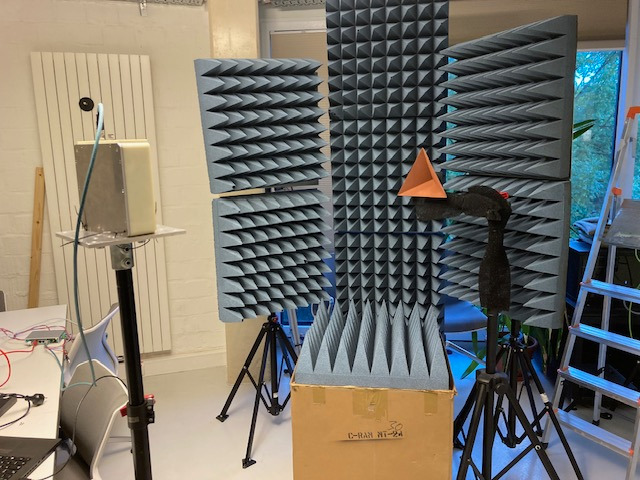
\includegraphics[height=0.25\textheight]{../figures/aufbau1.jpg}
    \caption{Measurement Setup}
    \label{fig:photo_setup}
\end{figure}
\begin{figure}
    \centering
    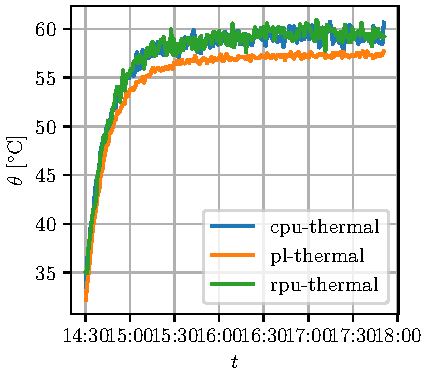
\includegraphics[height=0.25\textheight]{../figures/actual_temperature.pdf}
    \caption{Measured System Temperature After Startup}
    \label{fig:act_temp}
\end{figure}

Due to the geometry of the setup, the runtime of each transmitted wavefront should be identical.
Thus, the ideal deramped signal should be of a single, constant frequency and without inter-channel phase differences.
\begin{figure}
    \centering
    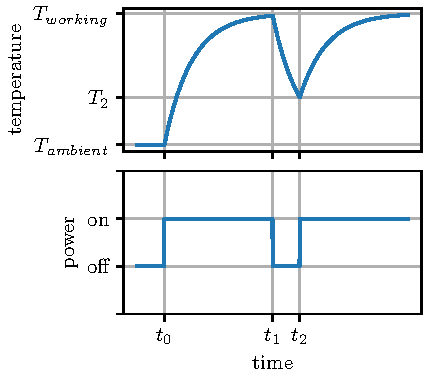
\includegraphics[height=0.25\textheight]{../figures/expected_temperature.pdf}
    \caption{Expected System Temperature over Time for Interrupted Power}
    \label{fig:exp_temp}
\end{figure}
In practice, the reflector peak will have a certain bandwidth,
and other peaks at higher and lower frequencies will be present due to incomplete shielding and/or unwanted reflections.
Also, the reflector peak may wander if the setup geometry moves. \\
For analysis, system runtime and temperature cannot be considered independent variables, as illustrated in figure \ref{fig:exp_temp}:
The system starts at ambient temperature, heating up and approaching a stable operating temperature on turning on ($t_0$), and cooling back down after turning off ($t_1$). \\
\subsection{Results}
\begin{figure}[h]
    \centering
    \begin{subfigure}[t]{.45\textwidth}
        \centering
        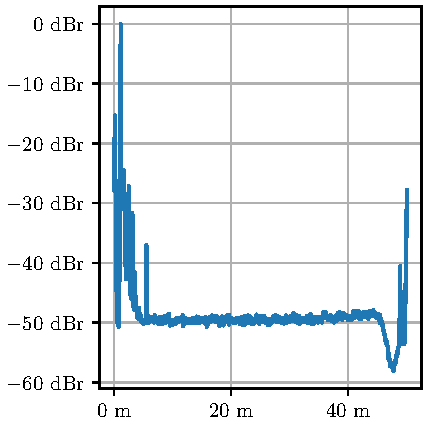
\includegraphics[width=\textwidth]{../figures/interference.pdf}
        \caption{Complete Spectrum}
    \end{subfigure}
    \begin{subfigure}[t]{.45\textwidth}
        \centering
        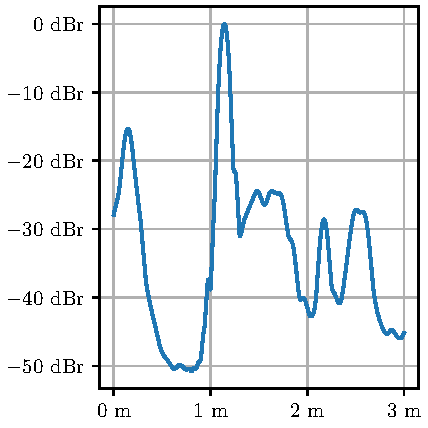
\includegraphics[width=\textwidth]{../figures/interference_zoom.pdf}
        \caption{Zoomed in}
    \end{subfigure}
    \caption{Mean Intensity Spectrum}
    \label{fig:avg_intensity}
\end{figure}
\subsubsection*{Preprocessing and Analysis}
Because of the aforementioned imperfections in the experiment, some preprocessing is required to analize the systematic offsets present in the radar signal.
Multiple additional peaks in the spectrum are visible in figure \ref{fig:avg_intensity}; indeed, the maximum peak is not even caused by the reflector.
It is therefore necessary to limit the analysis to only the FFT-bin at the maximum of the peak caused by the reflector.

The measurement environment also exhibits some minor changes in temperature and humidity, which can result in the geometry to shift by a few millimeters.
This shows by the spectral maximum shifting over time, as seen in figure \ref{fig:refldist}.

\begin{figure}
    \centering
    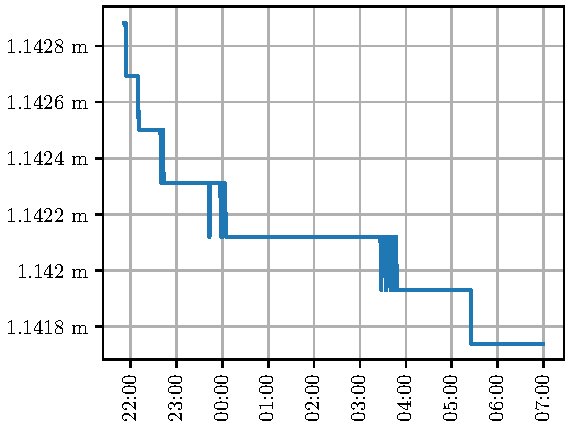
\includegraphics[height=0.25\textheight]{../figures/refldist.pdf}
    \caption{Change in reflector distance as measured by iMCR}
    \label{fig:refldist}
\end{figure}

In the following analysis, the main metric is the complex ratio of the maximum FFT-bin to its initial value.
Using a logarithmic representation  of this ratio, it can be represented as a level difference [\unit{\decibel}] and a phase difference [\unit{\degree}].

\subsubsection*{Effects of System Temperature and Runtime}

Multiple measurements have indicated that, while the amplitude rarely varies by more than \SI{1}{\decibel}, the phase is not as stable over time.
Typically, the mean phase drifts by up to \SI{50}{\degree} in the hours after system startup, with the rate of change reducing after around four hours.
However, it has to be noted that there is no clear correlation between phase drift and temperature:
the phase continues to drift after the system temperature stabilizes;
the reduction in drift only occurs hours after the system has reached a stable temperature of approximately \SI{60}{\celsius}.

\begin{figure}
    \centering
    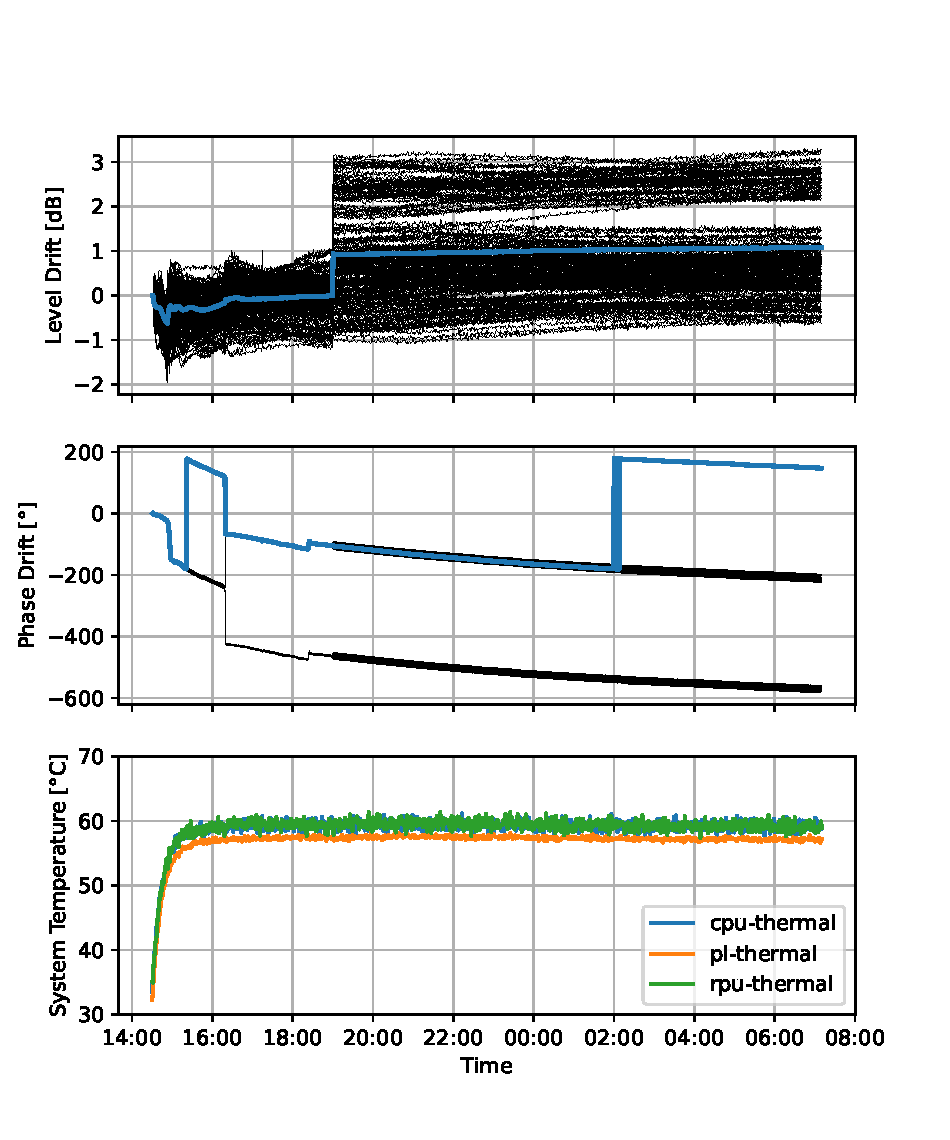
\includegraphics[width=\textwidth]{../figures/meas_23-10-09_phase_drift.pdf}
    \caption{Recorded drift over night}
    \label{fig:weekend}
\end{figure}

\subsubsection*{Effects of Self-Calibration}
As described in the specification, the AWR2243P-chips undergo a self-calibration upon initialization.
This initialization can be triggered by either restarting the entire system or by re-writing the configuration registers on the radar chips.
Indeed, this initial calibration can be observed in the data (cf. \ref{fig:restart}).
After the connection with the radar has been re-established, the following effects are visible:
\begin{itemize}
    \item slightly increased level: the level in each channel increases by approximately \SI{0.3}{\decibel}
    \item increased incoherence: after re-starting the system, the drift in both level and phase is distributed more broadly
    \item mean phase: the mean phase drift changes by up to \SI{5}{\degree}
\end{itemize}

\begin{figure}
    \centering
    \includegraphics[width=\textwidth]{../figures/meas_23-10-30_phase_drift.pdf}
    \caption{Recorded drift and temperature with system restart}
    \label{fig:restart}
\end{figure}


\subsubsection*{Differences between Antenna Pairs}
Comparing the amplitude recorded by all antenna pairs, no channel in particular stands out.
When looking at the different channels phase drifts, it can be seen that the array becomes less coherent over time.
The distribution of phase shift across channels seems roughly gaussian, with increasing variance over time.
No antenna pair seems more prone to incoherence than the rest:
across measurements, the maximum outlier (in terms of divergence from the mean phase) cannot be associated with a chip or antenna.

\subsubsection*{Effects of the Recorded Frequency and Angle}
- ?
\subsubsection*{Conclusion}
The systematic offsets of the system are now better described.
While the amplitude of the measured signal is relatively stable, the phase is affected more strongly.
All channels' phases drift from both their initial value and each other over time.
It can also be demonstrated that restarting the radar frontend has an effect on the phase, since the frontend undergoes an automatic calibration each time.
No clear bias within the array has been found, seeing that across multiple measurements, all channels seem to be affected similarly.

Overall, it has been demonstrated that the radar system cannot be considered ideal and
its imaging fidelity will be affected by the growing incoherence during long runtimes.
Furthermore, restarting the system will change the systematic offsets due to the automatic calibration of the radar frontend hardware.
Adaptive online calibration would be required to deal with these effects. \\

To limit the scope of this thesis, the focus is set on the offline-part of the calibration process.
Since the speed at which the array incoherence grows is limited, it can be considered static during sufficiently short measurements.
Also, because these offsets are affected by the automatic calibration of the system, the calibration has to be repeated on every startup.

\section{Antenna Characteristics}
\label{sec:calibration}

In this section, the array's antenna gains are measured and then analyzed.
The measured antenna gains can then directly be employed as weights for the backprojection algorithm,
resulting in a calibrated array.
A subset of the extrated paramters can also be employed for offline calibration when using FFT-based imaging.


\subsection{Experiment Setup}
The experiment done to measure the array's antenna gain patterns was conducted outdoors.
This is preferable because the experiment requires more physical space than the previous stability analysis,
and of course minimal interfering clutter in that space.
As shown in \cref{fig:setup_rotating}, the sensor is mounted on a vertical rotating axis,
and a corner reflector is placed in front of the sensor.
Rotating the axis allows the sensor to observe the corner reflector from multiple angles, while retaining a fixed distance.
Doing this can be used to measure the antenna gains in azimuth;
to measure the antenna gains in elevation, the sensor is mounted on the same axis to rotate around its horizontal axis.
These two measurements are repeated for multiple reflector distances.

While the relative position of the rotating axis can be recorded with a decent resolution of around \SI{0.01}{\degree},
the absolute positioning of the reflector is hard to achieve with the same accuracy.
The sensor itself can however be used to improve positioning accuracy:
during setup, the phase of the peak caused by the reflector
is extracted with a similar method as in \cref{sec:stability_analysis} and displayed.
Mimimizing the phase differences between the array's channels by fine-tuning the reflector's position
ensures that it be located at boresight.
These measurements are repeated with multiple distances of the relector.\\
\begin{figure}[h]
  \centering
  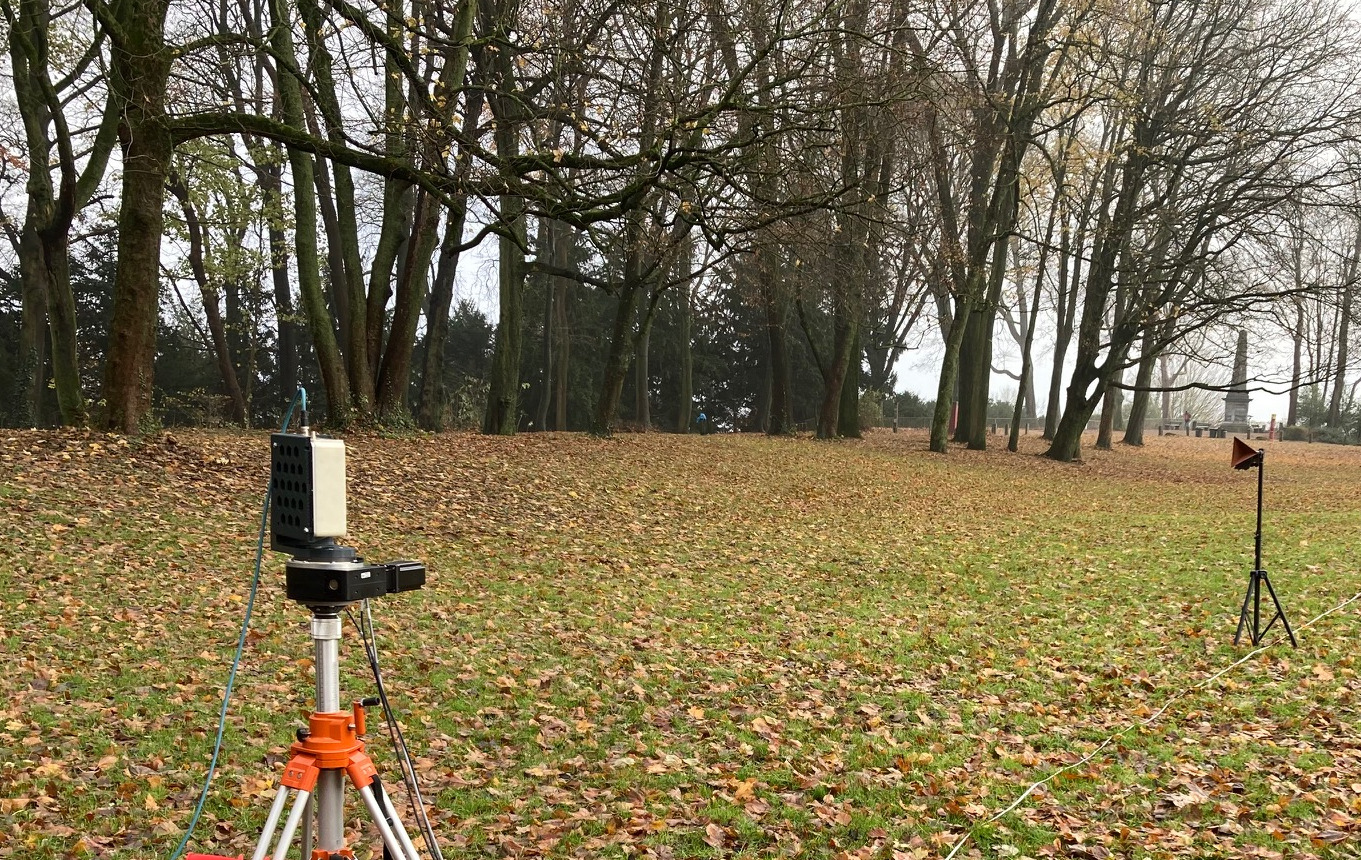
\includegraphics[width=0.6\textwidth]{../figures/setup_rotating.jpg}
  \caption{iMCR Antenna Gain Measurement Setup}
  \label{fig:setup_rotating}
\end{figure}

The field on which the experiment was set up is widely void of clutter, but not entirely.
Several trees and brushes are located at the edge of the scene.
Extra interference and reflections are caused by the floor.
It is also not perfectly level, varying in height by up to \SI{1}{\meter},
which means that the reflector is not always exactly at the same height.
The sensor mount also causes some problems [NEEDS DRAWING]:
when the sensor is mounted on its inside,
the rotational axis passes exactly through the antenna array's plane,
but some shading is occurs when the reflector is on the same side as the sensor mount's diagonal reinforcement.
When the sensor is mounted on the outside,
the rotational axis is no longer in the antenna array's plane,
adding complexity and inaccuracy to the subsequent analysis.

\subsection{Preprocessing and Analysis}
The objective of the subsequent analysis is to extract the antenna gains from the measured IF-signals.
In \cref{sec:single_channel_fmcw},
the the ideal deramped signal $y_{kl}[m]$ from channel $k$ at long-time index $l$
for a single reflector at position $\vec r_l$
is defined in \cref{eq:channel_gain} :
\begin{align*}
  y_{kl}[m] =  C_k(\vec r_l)e^{-j\omega_0\tau_{kl}}e^{-j\dot\omega\tau_{kl}mT_s}
\end{align*}
The square channel gain directly relates to the antenna gains $A_i$ and $B_j$
of the transmit antenna with index $i$ and the receive antenna with index $j$ that make up the channel:
\begin{align*}
  C_k^2 = \frac{P_{Rx}}{P_{Tx}}
  = G_{Tx}(\theta,\phi)  G_{Rx}(\theta,\phi) \frac{\sigma}{4\pi} \left(\frac{\lambda}{4\pi R_1 R_2}\right)^2
\end{align*}
For simplicity's sake, the following quantities are defined:
\begin{align}
  c_k(\theta,\phi) := \frac{C_k(r,\phi,\theta)}{\max |C_k(r,\phi,\theta)|}
\end{align}
will be called the \emph{channel characteristic}, and assumed to be constant in $r$ with $c_k(\theta,\phi) \in [0,1]$.
The \emph{antenna gains} are the relative maximum antenna gains of the transmit and receive antennas:
\begin{align}
  \underline A_i & :=  \frac{\max G_{Tx,i}(\theta,\phi)}{ G_{Rx,0}(\theta,\phi)}e^{j\psi_i}      \\
  \underline B_j & :=  \frac{\max G_{Rx,j}(\theta,\phi)}{ G_{Rx,0}(\theta,\phi)}e^{j\vartheta_j}
\end{align}
As defined in \cref{eq:kij}, each channel $k$ has a corresponding transmit antenna $i$ and a receive antenna $j$.
All antenna gains are defined with regards to the reference antenna, receive antenna 0.
They also include a phase offset which describe any mismatches in the individual antenna,
such as polarization, reflections in the antenna ports or length offsets in the transmission lines leading to them.

With that, the radar range equation can be rewritten as follows:
\begin{align*}
  \underline C_k^2 = \underline A_i \underline B_j c_k^2(\theta,\phi) e^{j2\left(\varphi_k-\omega_0\frac{R_1+R_2}{c_0}\right)}
  \frac{\sigma}{4\pi} \left(\frac{\lambda}{4\pi R_1 R_2}\right)^2
\end{align*}

The goal of the subsequent analysis is twofold:
to extract all parameters of the above signal model while identifying and removing interference through processing.

Limiting the analysis to a single range bin will work towards both reducing interference and extracting parameters:
ideally, the DFT spectrum of the IF signal consists of just a single peak,
weighted with the channel gain $C_k(\vec r)$ (see \cref{eq:y_fft}).
Thus, the channel gain can be extracted if the correct bin $\hat \Omega$ is picked:
\begin{align}
  \hat \Omega                                               & = \dot \omega \tau_k(\vec r_S)T_s              \\
                                                            & = \dot \omega \frac{R_1+R_2}{c}T_s             \\
  \Rightarrow \mathcal{F}_m\{y_k[m]\}(\Omega = \hat \Omega) & =    \underline C_k(\vec r_S) \label{eq:G_fft}
\end{align}

\subsection{Range Estimation}
\label{sec:range_est}


In order to improve the accuracy of the subsequent analysis, the exact position of the reflector is estimated from the radar data.
To do this, numerical optimization is employed to find the parameter set
$\hat R_s, \hat \theta_s, \hat \epsilon$ that minimizes the difference between
a range estimate $\hat R_{k,l}$ and the range spectral peak $R_{k,l}$ for all channels $k$ and recorded orientations $l$:
\begin{align}
  R_{k,l} = \arg \underset{r}{\max}\,\mathcal{F}_m\{y_{k,l}[m]\}\left(\Omega = \frac{N_{fft}r}{R_{max}}\right)
\end{align}

The range estimate $\hat R_{k,l}$ is determined geometrically from the distances of each channel's
transmit and receive antenna to the reflector. If the sensor is mounted to rotate in azimuth,
the range depends on the rotation angle $\theta_l $:

\begin{align}
  \hat R_{k,l}   & = \frac{\| \vec r_{TX,k} - \vec r_S(l) \|+\| \vec r_{RX,k} - \vec r_S(l) \|}{2}
  \\
  \vec{r}_{TX,k} & = \begin{bmatrix}
                       x_{TX,k} \\ y_{TX,k} \\ \hat \epsilon
                     \end{bmatrix},
  \vec r_{RX,k}       = \begin{bmatrix}
                          x_{RX,k} \\ y_{RX,k} \\ \hat \epsilon
                        \end{bmatrix},                                                                                        \\
  \vec r_S(l)    & = \begin{bmatrix}
                       (\hat R_S-\hat \epsilon) \text{sin}(\hat \theta_S-\theta_l) \\ 0 \\ (\hat R_S-\hat \epsilon) \text{cos}(\hat \theta_S-\theta_l)
                     \end{bmatrix},
\end{align}
If the sensor is mounted to rotate in its elevation, the reflector appears to move depending on the rotation in elevation $\phi$.
For a given rotation angle $\phi_l$, the reflector is located at
\begin{align}
  \vec r_S(l) & = \begin{bmatrix}
                    0 \\ (\hat R_S-\hat \epsilon) \text{sin}(\hat \phi_S-\phi_l) \\ (\hat R_S-\hat \epsilon) \text{cos}(\hat \phi_S-\phi_l)
                  \end{bmatrix},
\end{align}

In our setup, a signal is recorded with $\theta$ (or $\phi$, respectively) from \SIrange{0}{180}{\degree},
with the reflector located at roughly $R_S = \{2,8,18,32\}\si{\meter}$ and either $\theta_S = \SI{90}{\degree}$ or $\phi_S = \SI{90}{\degree}$. \\

With this, the loss $\mathcal L$ can be defined as the mean square difference between $\hat R$ and $R_{p}$,
the mean being computed as the average over all $K$ channels and $L$ sensor rotations:
\begin{align}
  \mathcal L(\hat R_s, \hat \theta_s, \hat \epsilon)
  = \frac{1}{KL}\sum_{l=0}^{L-1} \sum_{k=0}^{K-1} ( R_{k,l} - \hat  R_{k,l}(\hat R_s, \hat \theta_s, \hat \epsilon))^2
\end{align} \\

\begin{figure}[h]
  \centering
  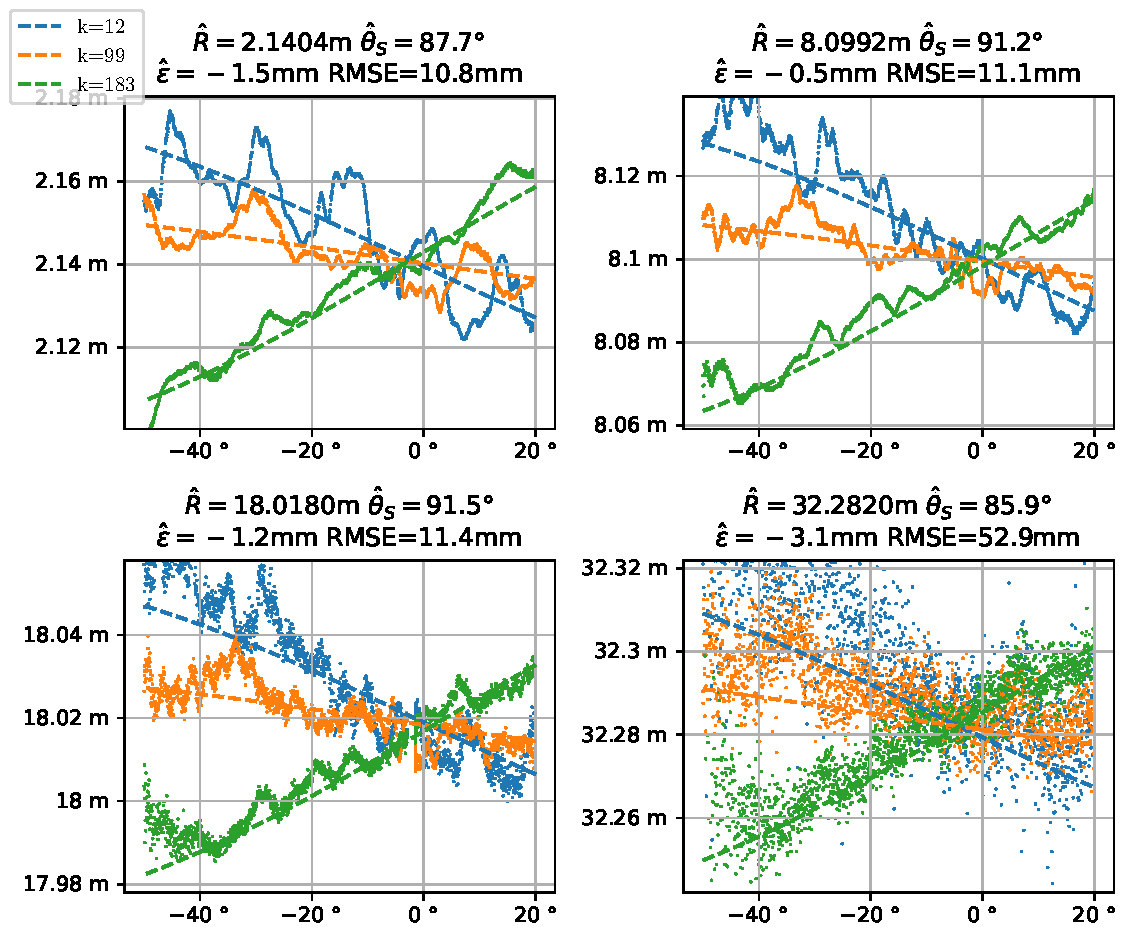
\includegraphics[width=\textwidth]{../figures/reflpos_estimate.pdf}
  \caption{Example Optimization Results}
  \label{fig:reflpos_estimate}
\end{figure}

\cref{fig:reflpos_estimate} shows the result of 100 iterations at an adaption rate of 0.05 at the example of three different channels,
comparing the measured spectral peaks (shown as points) to the estimated position (dotted line) of the reflector.
Only a subset of orientations is used for the estimate,
namely \SI{-50}{\degree} $<\theta_l-$\SI{90}{\degree}$<$ \SI{20}{\degree}. \\

For the first three measurements, the peak location oscillates around the estimate by \SIrange[range-units=single]{1}{2}{\cm}.
The \emph{root mean square error} (RMSE) is reduced to \SI{11}{\mm}.
Due to the decreasing signal level received from higher distances,
the fourth measurement has a higher relative noise level, resulting higher movement of the spectral peaks, and hence a much higher RMSE.

\newpage

\begin{figure}
  \centering
  \begin{subfigure}{\textwidth}
    \centering
    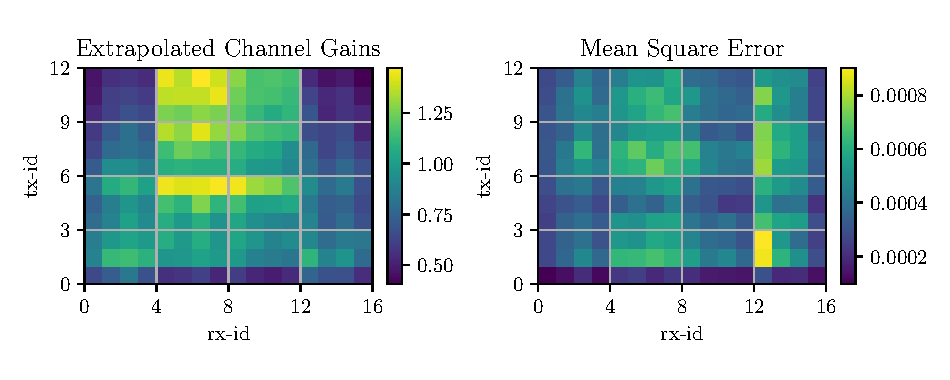
\includegraphics[width=\textwidth]{../figures/amplitude_linreg.pdf}
    \subcaption{Resulting Coefficents}
    \label{fig:amp_linreg}
  \end{subfigure}
  \vspace{1cm}
  \begin{subfigure}{0.5\textwidth}
    \centering
    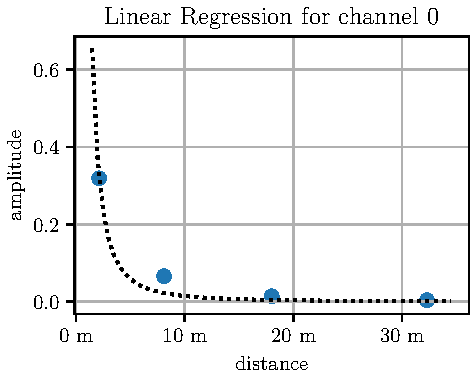
\includegraphics[width=\textwidth]{../figures/ch0_amplitude_linreg.pdf}
    \subcaption{Example: channel 0}
    \label{fig:ch0_amp_linreg}
  \end{subfigure}
  \caption{Linear Regression of Transmission Coefficients}
\end{figure}
\subsection{Amplitude}
\label{sec:amplitude}
First, the recorded amplitudes are analyzed, beginning with the influence of the angle of arrival.
To do this, each channel's range FFT spectrum's amplitude is evaluated at the respective calculated peak location $\hat \Omega$,
and then normalized by dividing it by its maximum.

The first parameters to extract are the three real-valued factors $A_i$, $B_j$ and $c(\theta,\phi)$.
First, we define a quantity that will be referrred to as the transmission coefficient:
\begin{align}
  \alpha_k = \sqrt{\frac{\sigma}{4\pi}A_iB_j}
\end{align}
Since the channel characteristic has been constrained to $[0,1]$,
the transmission constant can be expressed in terms of the two distances
$R_1 = \|\vec r_s - \vec r_{Tx,k}\|$ and $R_2 = \|\vec r_s - \vec r_{Rx,k}\|$, and other known constants: \\
\begin{align}
  \underset{\theta,\phi}{\text{max}} |\underline C_k(R,\theta,\phi)|
   & = \alpha_k\frac{\lambda}{4\pi R_1R_2} = \alpha_k \frac{1}{R_1R_2} \frac {2\pi c_0}{\omega}          \\
   & = \alpha_k \frac{1}{4\pi R_1R_2} \dfrac {2\pi c_0}{\omega_0 +  \dot \omega \frac{R_1+R_2}{c_0}}     \\
   & = \alpha_k \dfrac{c_0^2}{2R_1R_2\left(\omega_0c_0 +  \dot \omega (R_1+R_2)\right)} \label{eq:max_G}
\end{align}

With that, an estimate of the transmission coefficient $\hat \alpha_k$ can be obtained via linear regression.
An example linear regression is shown in \cref{fig:ch0_amp_linreg},
and the resulting estimates with their standard deviations are summarized in \cref{fig:amp_linreg}.

Having estimated the channel gains, we can now turn to analysing the channel characteristics.
Assuming the omptimal range bin $\hat \Omega$ is evaluated each time, we get
\begin{align*}
  \left|\mathcal{F}_m\{y_k[m]\}(\Omega = \hat \Omega)  \right| =  |C_k(\vec r)|
\end{align*}
Dividing that by the maximum gain (\ref{eq:max_G}) yields
\begin{align}
  \frac {|C_k(\vec r)|}{\underset{\theta,\phi}{\text{max}} |C_k(R,\theta,\phi)|}  = c_k(\theta,\phi)
\end{align}

\begin{figure}
  \centering
  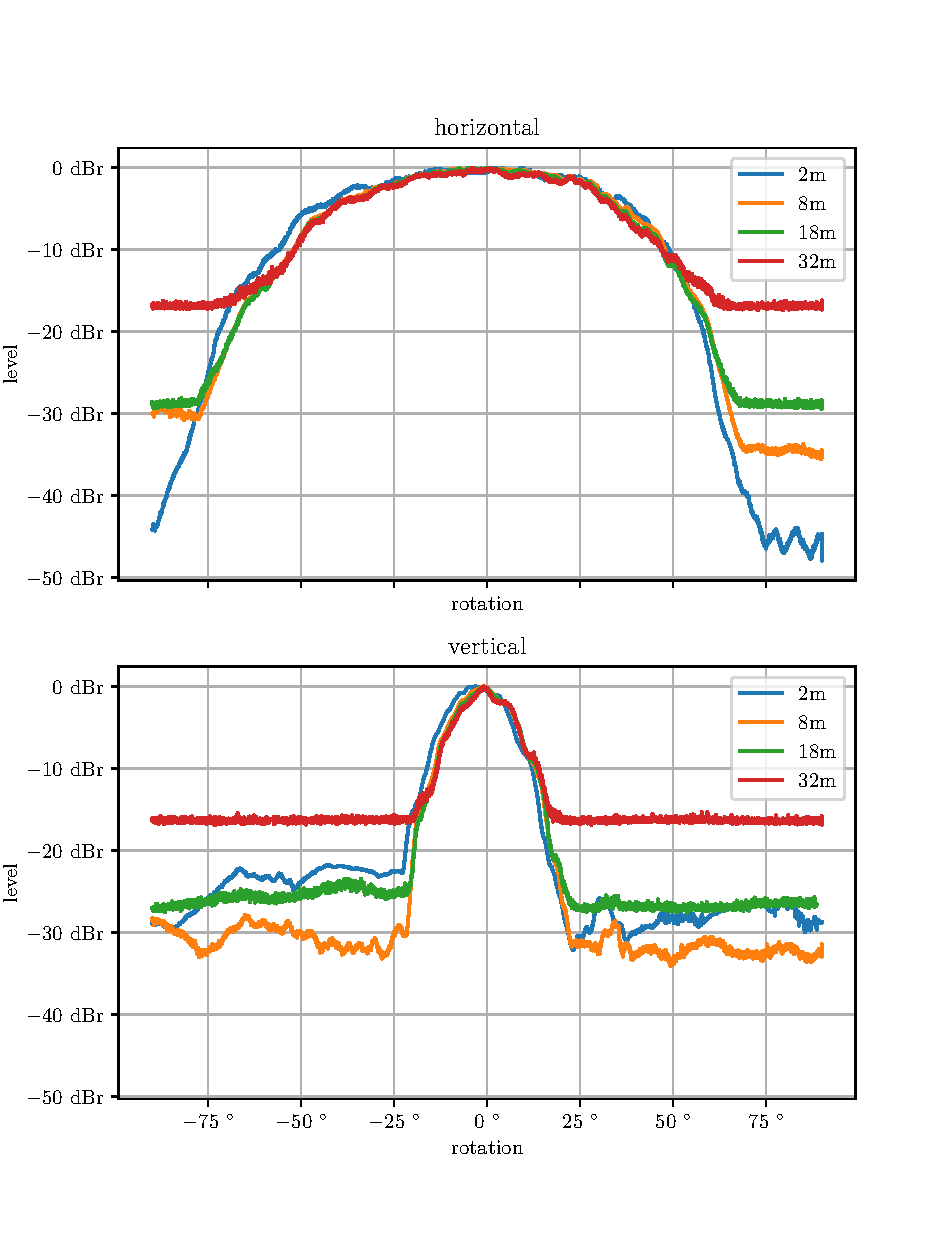
\includegraphics[width=\textwidth]{../figures/mean_amp.pdf}
  \caption{Mean Channel Characteristic for multiple reflector distances}
  \label{fig:mean_amp}
\end{figure}

\cref{fig:mean_amp} provides an overview by displaying the mean channel characteristic for each measurement.
It can be seen that the gain is strongest when the target is directly in boresight,
tapering off when the target is off-center. The reduction in gain is stronger when the target
moves off to the side in the elevation, than in azimuth. While the target remains stronger
than background noise up until an azimuth angle of around \SIrange{-75}{+75}{\degree},
it can only be seen in an elevation angle sector from \SIrange{-25}{+25}{\degree}.

The graphs of the horizontal measurements appear slightly asymmetrical, an effect which is investigated in the following.

\begin{figure}
  \centering
  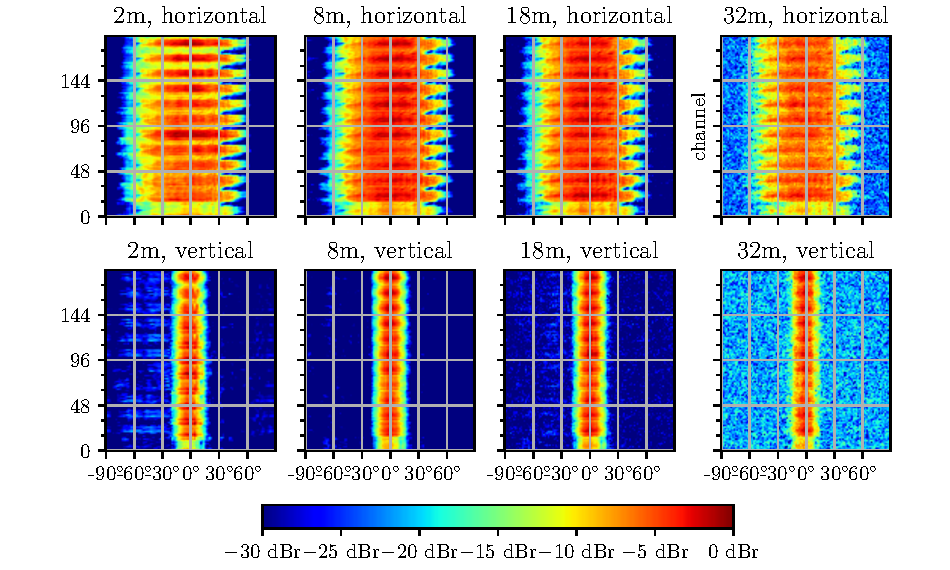
\includegraphics[width=\textwidth]{../figures/channel_amp.pdf}
  \caption{Channel-wise amplitude for multiple distances}
  \label{fig:chan_amp}
\end{figure}

A possible explanation for the asymmetry is the sensor mount,
which protrudes out on the right side of the array,
attenuating the signal received by antennas on that side when the reflector is behind said protrusion.

Investigating the individual channel gains (c.f. \ref{fig:chan_amp}) gives a first indication:
the asymmetry is most pronounced when comparing the range of \SIrange{30}{60}{\degree}
to its counterpart of \SIrange{-30}{-60}{\degree} for the horizontal measurements.
Namely, in the former range, the gain seems to oscillate every 16 channels.

\begin{figure}
  \centering
  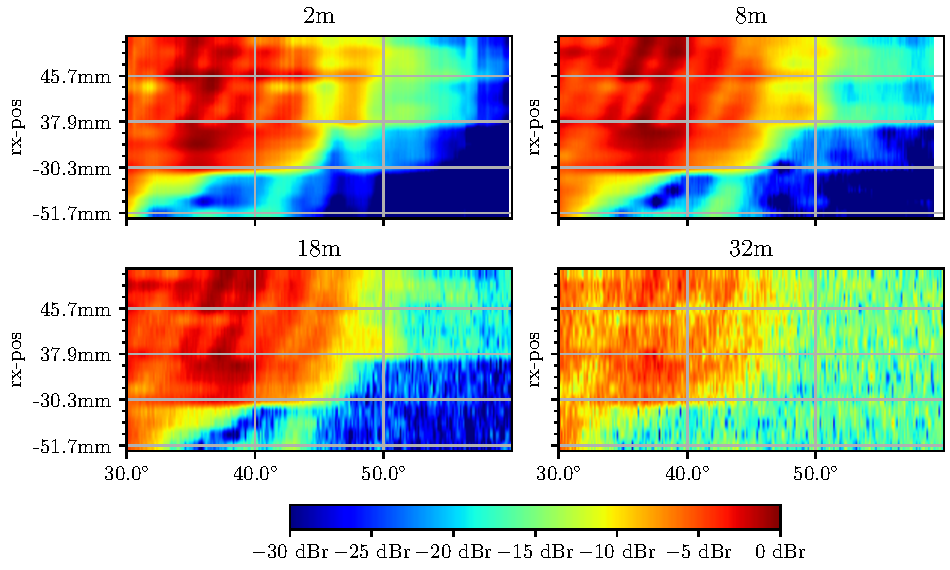
\includegraphics[width=\textwidth]{../figures/channel_amp_tx0.pdf}
  \caption{Channel-wise amplitude for multiple distances, channels arranged by Rx antenna position, only Tx antenna 0 active}
  \label{fig:chan_amp_tx0}
\end{figure}

To explore further, \cref{fig:chan_amp_tx0} zooms in on one period.
It shows the channel gain of the horizontal measurements for angles \SIrange{30}{60}{\degree}
of the channels in which transmit antenna 0 is active, arranged by the horizontal position of the receive antenna, from left to right.
It can now be seen that the channel gain of antennas closer to the sensor mount's protrusion drops
in amplitude at lower angles than that of the antennas further away from it,
confirming that the sensor mount is responsible for the asymmetry.
To get a more accurate estimate of the channel characteristics,
the measurements have to be repeated with the sensor mounted on the outside.\\

With this, the individual antenna gains and the channel characteristics have been extracted from the data.
In the next step, the recorded phases are analyzed. \\

\newpage
\subsection{Phase Estimation Techniques}

The first step in extracting the phase parameters from the recorded data is yet again
evaluating the signal's DFT phase at the optimum range bin $\hat \Omega = \frac{ N \dot \omega}{c_0 f_s}\hat R_k$,
which according to (\ref{eq:G_fft}) should ideally yield
\begin{align}
  \Phi_k(\vec r_S) :     & = \arg\, \mathcal{F}_m\{y_k[m]\} (\hat \Omega(\vec r_S)) \\
                         & =    \arg\,\underline C_k(\vec r_S)                      \\
                         & = \omega_0\tau_k(\vec r_S) + \varphi_k                   \\
  \text{with } \varphi_k & = \frac{\psi_{i}+\theta_{j}}{2}
  \text{ and } \tau_k    = \frac{2R_k}{c_0}
\end{align}

However, this part of the analysis is highly dependent on the accuracy of our assumptions,
specifically the distance between reflector and sensor.
The phase $\Phi_k(\theta) = \omega_0 \frac{2R_k(\theta)}{c_0} + \varphi_k$ changes immensely with small changes in said distance.

To illustrate, a change of $\Delta R_k = \SI{1}{\mm}$ would cause approximately the folowing phase shift:
\begin{align*}
  \Delta\Phi_k & = \omega_0 \frac{2\Delta R_k}{c_0}                                            \\
               & = 2\pi \cdot \SI{77e9}{\Hz} \cdot \frac{2\cdot\SI{1e-3}{\m}}{\SI{3e8}{\m/\s}} \\
               & = 0.5133 \pi = \SI{92.4}{\degree}
\end{align*}
The range estimate made in \cref{sec:range_est} had an RMSE of at least \SI{11}{\mm},
which introduces high uncertainty into the phase evaluation. \\

Another method to extract the phase from the recorded data is evaluating the FFT at the spectral peak,
which was the method of choice in \ref{sec:stability_analysis}.
Which method copes better with the presence of interference?
In the following, we will illustrate the effects of interference with a simulated signal,
as well as the impact of the interference on the two estimation methods accuracy.

Consider the signal received by an arbitray channel of the array $y(t,\theta)$.
Its frequency slowly changes as the orientation angle $\theta$;
for simplicity's sake, let the frequency shift linearly with $\omega(\theta)=2\pi (\SI{5}{\MHz} + \SI{1}{\MHz} \cdot \theta), \theta \in [-1,+3]$.
This results in our ideal signal
\begin{align*}
  y_{id}(t=mT_s,\theta) = 1 \cdot e^{-j\omega(\theta)mT_s}
\end{align*}
Introducing a source of interference with constant frequency $\omega_0$ and the amplitude $0.1$,
as well as a gaussian noise source $n(t,\theta) \sim \mathcal{N}(0;0.001)$, we get

\begin{align*}
  y(t=mT_s,\theta) = 1 \cdot e^{-j\omega(\theta)mT_s} + 0.1 \cdot e^{-j\omega_0 mT_s} + n(t,\theta)
\end{align*}

The spectrum of the ideal signal $Y_{id}(\Omega, \theta)$ and the degraded signal $Y(\Omega,\theta)$,
calculated with an $N=2048$ point FFT with $M=512$ samples in long-time, each corresponding to a different angle $\theta$,
is shown in fig. \ref{fig:interference_test_spectrum} in amplitude and phase.
\begin{figure}[h]
  \centering
  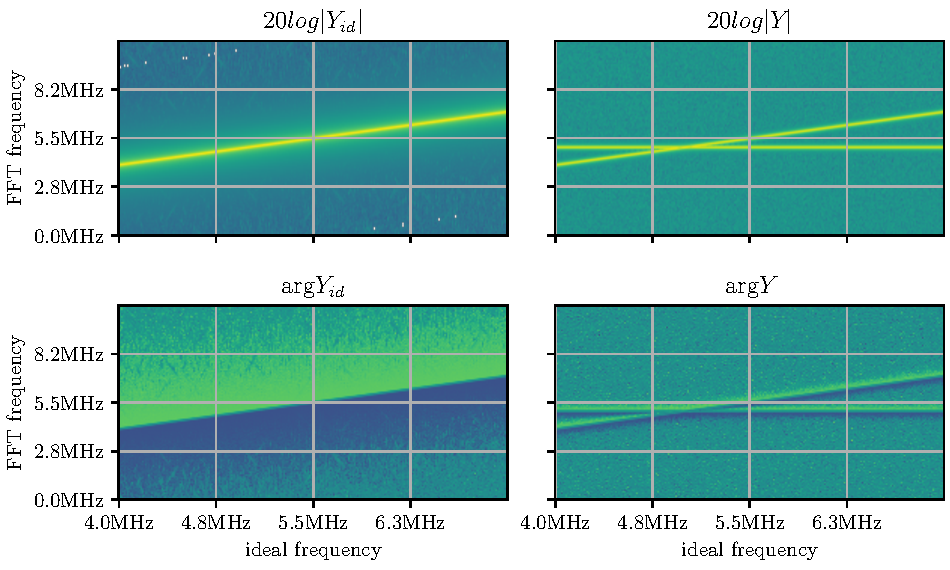
\includegraphics[width=\textwidth]{../figures/interference_test_fft.pdf}
  \caption{Spectra of example signal $Y$ and $Y_{id}$}
  \label{fig:interference_test_spectrum}
\end{figure}
The location of the both signals' spectral maxima can be seen in fig. \ref{fig:interference_test_peak},
showing that the interference causes the spectral maximum to move from its ideal location. \\
\begin{figure}
  \centering
  \begin{subfigure}{0.49\textwidth}
    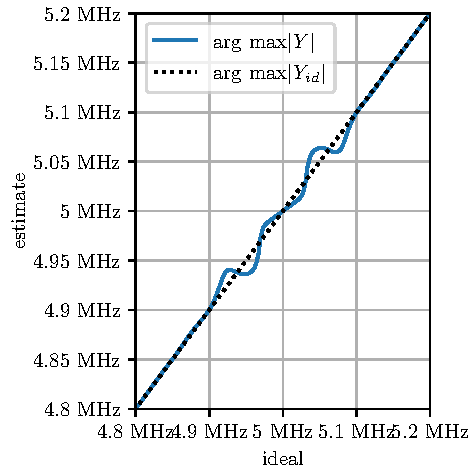
\includegraphics[width=\textwidth]{../figures/interference_test_peak.pdf}
    \subcaption{Peak Frequency}
    \label{fig:interference_test_peak}
  \end{subfigure}
  \hfill
  \begin{subfigure}{0.49\textwidth}
    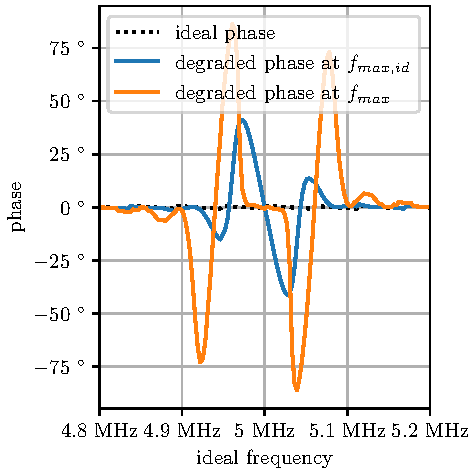
\includegraphics[width=\textwidth]{../figures/interference_peak_phase.pdf}
    \caption{Phase at peaks}
    \label{fig:interference_peak_phase}
  \end{subfigure}
  \caption{Extracting Phase from example spectra $Y$ and $Y_{id}$}
\end{figure}
\cref{fig:interference_peak_phase} finally shows the effect of interference on the phase.
We compare the phase of the ideal signal to phase of the degraded signal,
which is evaluated at both the ideal and the degraded signal's spectral maxima.
It can be seen that the latter method's phase diverges much more strongly from the ideal phase than that of the former,
and should therefor be preferred in the subsequent analysis. \\

\newpage
\subsection{Phase Analysis}
\label{sec:phase_analysis}
\begin{figure}
  \centering
  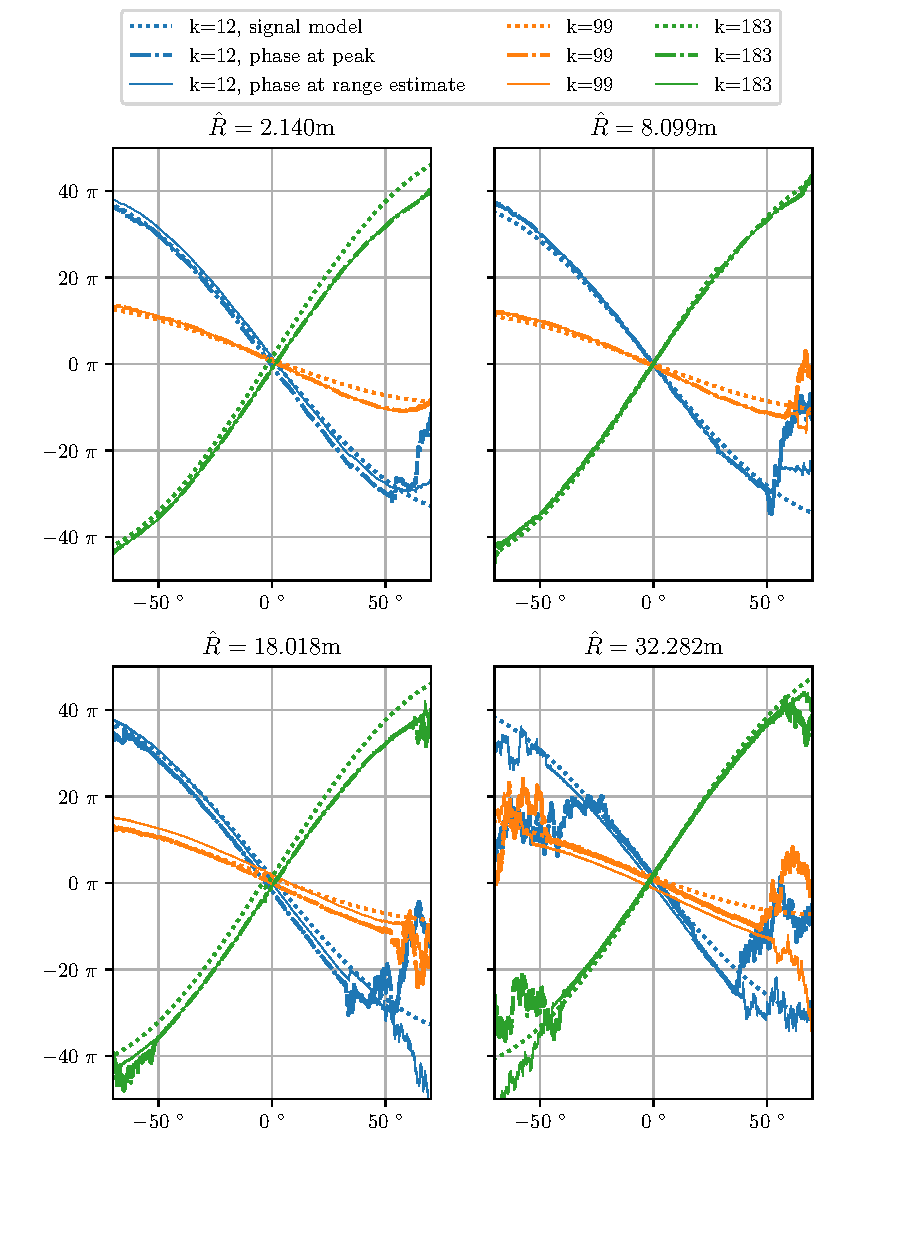
\includegraphics[width=\textwidth]{../figures/phase_estimates.pdf}
  \caption{Extracted Phase from measured signal, compared to signal model}
  \label{fig:measured_peak_phase}
\end{figure}
With knowledge of the robustness of our phase estimation against range estimation errors,
the task of extracting the phase parameters can be continued.
For better legibility of any graphs generated from the signal,
the phase of any given channel will be unwrapped from its original domain of $\theta \in [-\pi+\theta_s, \pi+\theta_s]$ such that no discontinuities
are visible when plotting phase against sensor orientation, while maintaining the original phase for $\theta = \theta_s$.

To assess the performance of the two techniques introduced in the previous section,
\cref{fig:measured_peak_phase} shows how they each compare to the signal model
\footnote{
  In this case, the signal model shown for comparison assumes that $\varphi_k = 0,\, \forall 0 \leq k<K$.
  Thus, the phase shown here is directly proportional to the estimated range $\hat R_k$:
  $$
    \hat\Phi_k(\theta) = \omega_0 \tau_k + 0 =  \frac{\omega_0}{c_0}2\hat R_k(\theta).
  $$
} for a few selected channels.
As it turns out, while being theoretically less robust against interference,
the phase evaluated at the signal peak is much smoother and matches our signal model much more closely. \\
\begin{figure}
  \centering
  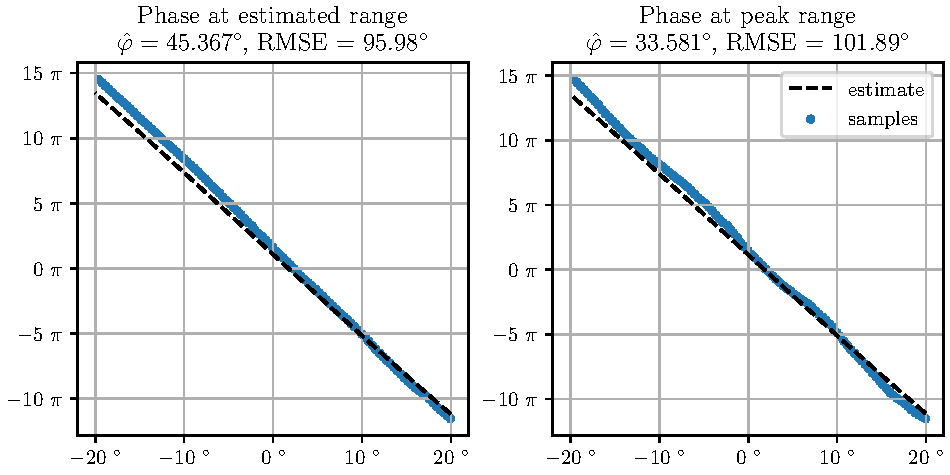
\includegraphics[width=\textwidth]{../figures/ch12_phase_linreg.pdf}
  \caption{Example: Channel 12 Phase Linear Regression}
  \label{fig:ch12_phase_linreg}
\end{figure}
Now, the channel phase offsets $\hat \varphi_k$ can be estimated using linear regression.
\cref{fig:ch12_phase_linreg} shows an example linear regression,
and the resulting channel phase offsets are shown in \cref{fig:phase_linreg}.
\begin{figure}
  \centering
  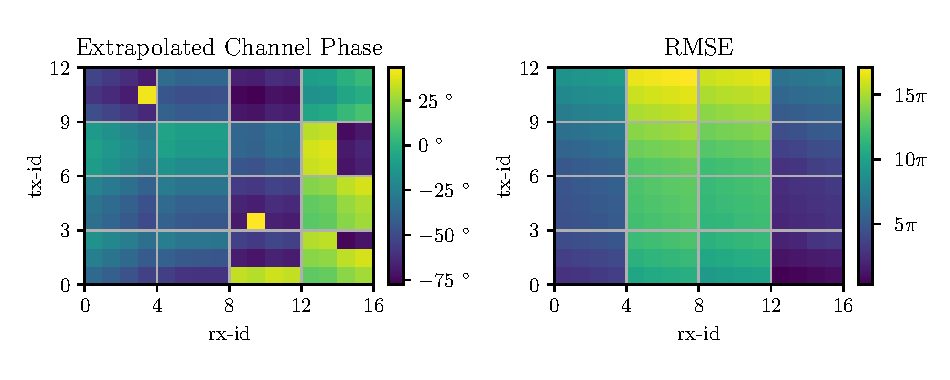
\includegraphics[width=\textwidth]{../figures/phase_linreg.pdf}
  \caption{Phase Linear Regression Overview}
  \label{fig:phase_linreg}
\end{figure}

\subsection{Antenna Separation}
To describe the array in terms of its channel gains is somewhat redundant.
As was defined in the underlying signal model, each channel gain $C_ke^{j\varphi_k}$ in actuality
just the product of the transmit and receive antenna gains, that is
\begin{align}
  C_k^2e^{j2\varphi_k} = A_i e^{j\psi_i} \cdot B_j e^{j\vartheta_j} \text{ for } k=N_{Tx}i+j
\end{align}

To more accurately describe the array,
the next step in our analysis is to estimate antenna gains of the receive and transmit array.
Multiple combinations were feasible, but the rightmost receive antenna 0 was defined as a reference antenna,
such that $B_0=1$ and $\vartheta_0 = 0$.

In the following, the channel gain amplitudes $\hat C_k$ that were estimated in \cref{sec:amplitude},
and the channel phase offsets $\hat \varphi_k$ from \cref{sec:phase_analysis}
are used to obtain estimates for the transmit and receive antenna parameters. \\

Thanks to the definition of a reference antenna,
the transmit antennas' amplitude and phase are easily obtained:
\begin{align}
  \hat A_i    & = \left.\hat C_k^2 \right|_{k=N_{Tx}i}     \\
  \hat \psi_i & = \left.\hat \varphi_k \right|_{k=N_{Tx}i}
\end{align}
With that, a least squares estimate for the remaining receive antennas' amplitude and phase is:
\begin{align}
  \hat B_{j\neq0}         & = \frac{1}{N_{Tx-1}} \sum_{i=1}^{N_{Tx-1}} \left. \frac{\hat C_k^2}{\hat A_i} \right|_{k=N_{Tx}i},        \\
  \hat \vartheta_{j\neq0} & = \frac{1}{N_{Tx-1}} \sum_{i=1}^{N_{Tx-1}} \left. \frac{2\hat \varphi_k}{\hat \psi_i} \right|_{k=N_{Tx}i}
\end{align}
The resulting antenna parameters are shown in tables \ref{tab:tx_gains} and \ref{tab:tx_gains}.
\begin{table}[h]
  \centering
  \begin{subtable}[t]{0.4\textwidth}
    \begin{tabular}{ccc}
      \toprule
      \textbf{Antenna} & \textbf{Gain}   & \textbf{Phase} \\
      \midrule
      0                & \num{4.134e+06} & 53.596°        \\
      1                & \num{7.847e+06} & 125.805°       \\
      2                & \num{7.363e+06} & 48.354°        \\
      3                & \num{6.169e+06} & -126.556°      \\
      4                & \num{5.445e+06} & -13.976°       \\
      5                & \num{6.815e+06} & -111.434°      \\
      6                & \num{5.174e+06} & -81.855°       \\
      7                & \num{3.962e+06} & 82.760°        \\
      8                & \num{3.517e+06} & 119.322°       \\
      9                & \num{2.831e+06} & 1.485°         \\
      10               & \num{2.291e+06} & 7.703°         \\
      11               & \num{2.158e+06} & -53.846°       \\
      \bottomrule
    \end{tabular}
    \subcaption{Tx Antennas}
    \label{tab:tx_gains}
  \end{subtable}
  \hfill
  \begin{subtable}[t]{0.4\textwidth}
    \begin{tabular}{ccc}
      \toprule
      \textbf{Antenna} & \textbf{Gain} & \textbf{Phase} \\
      \midrule
      0                & \num{1.000}   & 0.000°         \\
      1                & \num{1.463}   & -7.095°        \\
      2                & \num{1.676}   & -26.095°       \\
      3                & \num{1.426}   & 0.712°         \\
      4                & \num{3.797}   & -1.052°        \\
      5                & \num{3.635}   & 26.672°        \\
      6                & \num{3.999}   & 42.318°        \\
      7                & \num{3.703}   & -2.503°        \\
      8                & \num{3.391}   & 49.492°        \\
      9                & \num{2.867}   & -2.698°        \\
      10               & \num{2.751}   & 69.663°        \\
      11               & \num{2.631}   & -40.625°       \\
      12               & \num{1.393}   & 8.481°         \\
      13               & \num{0.987}   & -11.289°       \\
      14               & \num{1.129}   & -1.515°        \\
      15               & \num{0.820}   & -5.109°        \\
      \bottomrule
    \end{tabular}
    \subcaption{Rx Antenna Gains}
    \label{tab:rx_gains}
  \end{subtable}
  \caption{Estimated Antenna Parameters with Reference Rx0}
\end{table}

\subsection{Conclusion}
In this section, a method for estimating the antenna gains from real-world antenna measurements has been formulated
that optimizes the estimation's accuracy and robustness against interference.
The summarized steps are as follows:
\begin{enumerate}
  \item Setup the reflector in front of the sensor.
        For each distance to measure, center the reflector by observing a live readout of the phase at the spectral peak caused by the reflector,
        and positioning the sensor such that the phase differences between channels is minimal.
  \item From the measurements, extract the range of the spectral peak caused by the reflector for each channel and sensor orientation.
        Use numerical optimization to find a set of model parameters ($\hat R_s$, $\hat \theta_s$ or $\hat \phi_s$, and $\hat\epsilon$)
        that best matches the spectral peaks.
  \item Evaluate the amplitude of the spectrum at the frequency corresponding to the estimated range from the previous step.
        The maximum amplitude across all angles is the channel gain $C_k / R^2$,
        and the remaining attenuation is the channel characteristic $\hat c_k(\theta,\phi) \in [0,1]$.
        With linear regression across all measured distances, the channel gain at \SI{1}{\m} can be estimated.
        The estimated channel chararacteristic $\hat c_k(\theta,\phi)$ can indicate orientations with low SNR and/or high interference.
  \item Evaluate the phase of the spectrum at the frequency corresponding to the estimated range.
        Unwrap the phase of each channel such that the phase for $\theta = \hat \theta_s$ is in $[-\pi,\pi]$.
        Find the channel phase offset $\varphi_k$ that best matches the signal model to the measured phase.
  \item Separate each square channel gain $\hat C_k^2e^{j2\hat \varphi_k}$ into a transmit gain $A_i e^{j\psi_i}$ and a receive gain $B_j e^{j\vartheta_j}$.
        Do this by defining a receive antenna as a reference.
\end{enumerate}

Following these steps gives a decent estimate of the systems's physical properties with relatively lax requirements on the measurement itself.
This is especially desirable since \cref{sec:stability_analysis} demonstrated a need for frequent in-field calibration,
since the system parameters may change after restarting, and also shift over time. \\

More sophisticated methodology is required to achieve accurate measurements of the system.
Controlling the positioning of the reflector relative to the sensor more closely,
for example by placing the reflector on a linear axis,would greatly improve accuracy.

Interference sources in the environment would also have to be reduced.
This would involve moving the experiment to a more controlled environment,
such as a low-reflection room.

Another area of improvement lies in channel separation.
Since the reference antenna in the described method is not external,
but rather a part of the system under test,
all the results of our analysis indicate are relative differences between antennas.
Instead, an external antenna with known characteristics could replace the reflector,
allowing for more accurate measurements of the individual antennas' absolute characteristics.




\chapter{Image Reconstruction}
- recap results of last chapter
- restate motivation of imaging
- chapter overview

\section{PyTorch}
The algorithms implemented in this chapter are presented in the PyTorch framework.
As a machine learning framework, it provides accelerated tensor processing.
Tensors, ie.\ rectangular multidimensional arrays are a perfect fit to
describe the signals sent by the sensor and the subsequent signal processing.

Since a huge part of the operations in the imaging algorithms are parallelizable,
substantial performance gains can be achieved with the built-in parallel processing
of tensor operations in PyTorch.
While parallel processing on a CPU already substantially improves runtimes,
even better performance can be achieved with GPU-enabled parallel processing,
which is currently available using the CUDA-API on NVDIA GPUs.

To aid in understanding any code listings referenced in this chapter,
refer to a brief tutorial in section \ref{sec:pytorch_tutorial}
that discusses some key parts of PyTorch's syntax for tensor processing.

\section{FFT-Based Imaging}

The first imaging algorithm to be implemented is based on the FFT.
A detailed description of the algorithm can be found in section \ref{ssec:dft_imaging_theory},
but the following is an abrigded summary to reiterate the key principles.

The range is estimated by computing the FFT spectrum of each time signal;
due to the FMCW principle, the frequency of the received signal is directly related to its range.
Then, making the assumption of planar incident waves
as well as having calibrated the array to achieve coherence between channels,
the angle of arrival can be estimated using FFTs over the ULA subset of the sensor's virtual antenna array.
The resolution can be increased by zero-padding the signal before applying the FFT.
An example implementation in PyTorch is shown in code listing \ref{lst:fft_img}.

The function \verb|calc_image| returns a 3D-image of dimension $N_{range} \times N_{azimuth} \times N_{elevation}$.
Its input consists of \verb|data|, a time data tensor of dimension $M \times K$,
the calibration weights \verb|weights| of dimension $K$, and \verb|settings|, a dictionary of settings.
\verb|settings| is expected to contain the input and output dimensions,
the indices of the ULA subset of the virtual array with gaps indicated by $-1$,
as well as the window functions to be used in each FFT.

\subsection{Offline Calibration}
To compute the angle of arrival, the input signal has to be made coherent in phase.
This is done by deviding each channel's range spectrum $Y_k(\Omega)$ by the estimate channel gain $\hat C_k e^{j\hat \varphi_k}$.
As well as aligning the phases correctly, this also equalizes the channel gains. \\

\subsection{Direction of Arrival Accuracy}
\label{ssec:fft_doa}
This section aims to illustrate the theoretical capabilities of FFT-based DoA-estimation on the iMCR.
The directivity in azimuth and elevation is simulated for multiple distances to illustrate the impact of near-field conditions.
\\

For this, the input time signal is an ideal point source (see eqn.\ \ref{eqn:ideal_scatterer}),
located at $(R,\theta=0,\phi=0)$
% , degraded with CSCG\footnote{circularly symmetric complex Gaussian} noise
% $\underline{\mathbf n} \sim \mathcal{CN}(0, \sigma^2 \mathbf I) $ and 
assuming a constant antenna gain of $\underline G_k(r,0,0)=1 \,\forall r,k$:
\begin{align}
    \underline y_k[m] =  e^{-j\dot \omega \frac{2R}{c_0} m T_s}
    % + \underline n_k[m]
    ,\,k\in[0,K-1],m\in[0,M-1]
\end{align}
\\
The image is computed for multiple distances at resolution
$N_{range} = 1024, N_{azimuth} = 2048$ and $N_{elevation} = 8$.
and evaluated at the range and evaluation bin of the scatterer.
The resulting peaks in azimuth are shown in figure \ref{fig:fft_azm_peak}.
\begin{figure}[h]
    \centering
    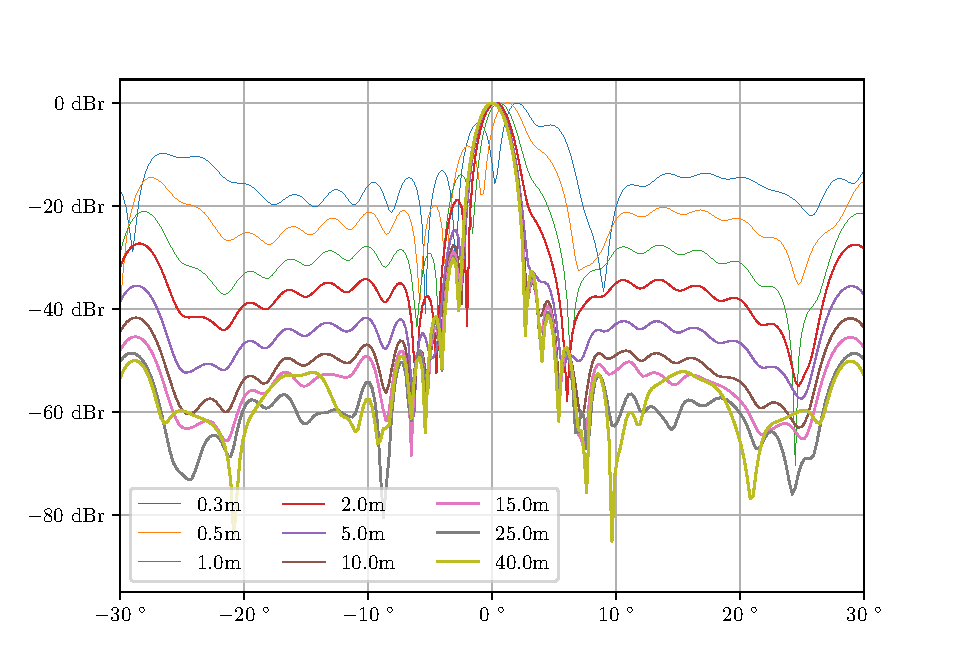
\includegraphics[width=\textwidth]{../figures/fft_azm_peak.pdf}
    \caption{iMCR FFT direction of arrival estimation: theoretical accuracy in azimuth for an ideal point scatterer at different ranges}
    \label{fig:fft_azm_peak}
\end{figure}

The Fraunhofer distance of the array can be computed from the wavelength $\lambda_0=$ \SIlist{3.944}{\mm}
and the virtual array's azimuth aperture $D_{azm} = 86 \frac{\lambda_0}{2}=$ \SI{16.96}{\cm}:
\begin{align}
    d_f  = \frac{2D_{azm}^2}{\lambda_0}
    = \SI{14.59}{\m}
\end{align}
It can be seen that for targets closer than $d_f$, the peak deteriorates in multiple ways.
The location of the peak moves to higher angles than the actual location of $\theta =$ \SI{0}{\degree}.
For targets at \SI{30}{\cm}, the peak has moved to $\theta =$ \SI{2.02}{\degree}.

In near-field conditions, the side lobe levels increase until their minimum only around \SI{20}{\dB} below the peak,
whereas in the far field, the minimum is \SI{60}{\dB} below the peak.

In far-field conditions, the main peak at $\theta =$ \SI{0}{\degree}
is clearly separated from its sidelobes by pronounced local minima.
The minimum to the right of the main peak starts to disappear below $d_f$,
and the peak to the right starts to merge with the main peak the closer the target gets.
The far-field half-power and quarter-power beamwidths are approximately
$\theta_{\SI{3}{\dB}}=$ \SI{1.9}{\degree} and $\theta_{\SI{6}{\dB}}=$ \SI{2.6}{\degree}, respectively. \\
\begin{figure}[h]
    \centering
    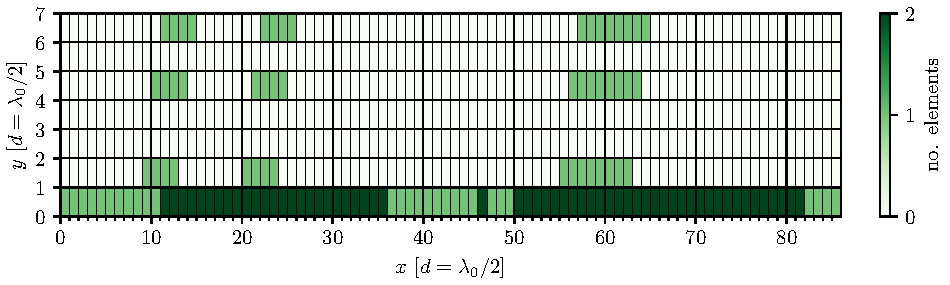
\includegraphics[width=\textwidth]{../figures/virt_array.pdf}
    \caption{iMCR virtual antenna array occupancy}
    \label{fig:virt_array}
\end{figure}

For direction of arrival estimation in azimuth, the 86-channel ULA subset of the array is well applicable to an FFT-based approach,
even with its reduced performance in near-field conditions.
Yet in elevation, such a ULA subset does not exist, as the array is sparse horizontally and vertically (c.f.\ \ref{fig:virt_array}).

To still use the FFT, an approach would be ``backfilling'' the array with zeros
to obtain a complete uniformly spaced rectangular virtual array.
The FFT is then computed over the collumns (c.f.\ \ref{fig:virt_array}) of this array,
each yielding a spectrum that is related to the direction of arrival in elevation.

A disadvantage of this approach is that it can cause substantial spectral leakage.
Our backfilled array $b[k] $ is mathematically equivalent
to applying a binary window function $w[k]$ to the ideal rectangular array $a[k]$:
\begin{align*}
    b[k]                   & =  w[k] \cdot  a[k]             \\
    \text{e.g.}\;  b[0..7] & = [b_0, b_1, 0,0,b_2,0,b_3,0 ], \\
    w[0..7]                & = [1,  1,0,0,1,0,1,0 ],         \\
    \text{and}\; a[0..7]   & = [a_0,a_1,a_2,\dots,a_7]
\end{align*}


However, this window function causes additional peaks to appear in the spectrum,
since multiplication in the time domain is equivalent to convolution in the frequency domain:
\begin{align*}
    \mathcal{F}\{b[k]\}[n] & = \mathcal{F}\{w[k] \cdot  a[k]   \}[n] \\
                           & = W[n] * A[n]
\end{align*}
In case of the example given above,
\begin{align*}
    |W[0..7]| = [4.00,\ 0.77,\ 1.41,\ 1.85,\ 2.00,\ 1.85,\ 1.41,\ 0.77]
\end{align*}

It would be possible to reduce the spectral leakage with deconvoltion algorithms.
To show the starting point for these algorithms,
the unadulterated spectral peak for targets at multiple distances is shown in figure \ref{fig:fft_elv_peak}.

\begin{figure}[h]
    \centering
    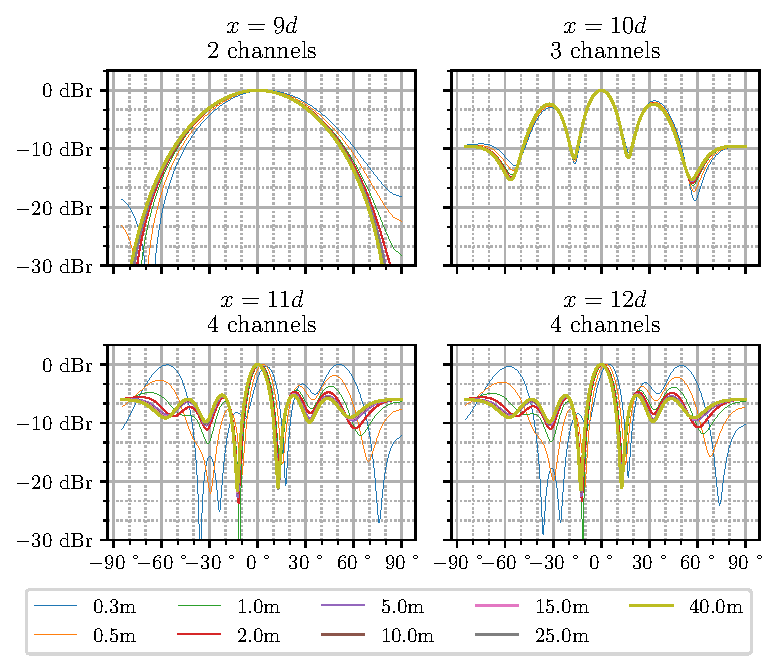
\includegraphics[width=0.8\textwidth]{../figures/fft_elv_peak.pdf}
    \caption{iMCR FFT-based direction of arrival: theoretical accuracy in elevation for an ideal point scatterer at different ranges and different array subsets}
    \label{fig:fft_elv_peak}
\end{figure}

It can be seen that the half-power beamwidth improves the more channels are included in the sub-array:
for two, three and four active channels, we approximately get
$\phi_{\SI{3}{\dB}}=$ \SIlist{60;14;12}{\degree}, respectively.

As the peak narrows, the spectrum contains more and more sidelobes.
For sub-arrays that include three channels, the side peaks are the strongest,
barely \SI{3}{\dB} less than the main peak. \\

The Fraunhofer distance of the array in elevation can be computed from the wavelength $\lambda_0=$ \SIlist{3.944}{\mm}
and the virtual array's maximal elevation aperture $D_{elv} = 7 \frac{\lambda_0}{2}=$ \SI{1.38}{\cm}:
\begin{align}
    d_f  = \frac{2D_{elv}^2}{\lambda_0}
    = \SI{9.66}{\cm}
\end{align}
The Frauenhofer distance in elevation is smaller than in azimuth by an order of magnitude.
Thus, all distances considered lie in the far-field,
and the shape of the peak should not change a lot over distance.

While this holds true for the two-- and three-channel case, if four channels are considered,
the shape does change with distance.

On the one hand, the location of the main peak moves to higher angles if the range is decreased.
On the other hand, the first two sidelobes decrease in amplitude,
while the third ones move towards $\phi=$ \SI{0}{\degree} and increase in amplitude.

TODO:

- Change Code listing

- Mention Taper Functions!!

- Conclude


\subsection{Test Image}
\label{ssec:fft_result}
To give an indication how well the theoretical capabilities of the FFT-based approach translate into real world applications,
a test scene was recorded. The sensor is placed in front of the old water tower on top of Lousberg, Aachen.
A reflector is placed slightly off-center at a distance of approximately \SI{6}{\m}.

The target 2D image spans a $24 \times$\SI{15}{\m} area in the horizontal plane,
with square pixels of edge length \SI{10}{\cm},
and the sensor located on one of the image's long sides, namely $[x,y] = [0,0]$.

It is constructed by first calculating the polar-coordinate FFT image at a resolution of $N_{range}\times N_{azimuth} = 2048 \times 512$.
% applying Hann window-functions in both fourier transforms.
The image can then be extracted from by selecting the appropriate range- and azimuth bins.
For calibration, previously measured antenna characteristics are used to improve the array's coherence.

Figure \ref{fig:fft_testimg} shows the resulting image with and without calibration.
\begin{figure}
    \centering
    \begin{subfigure}{0.8\textwidth}
        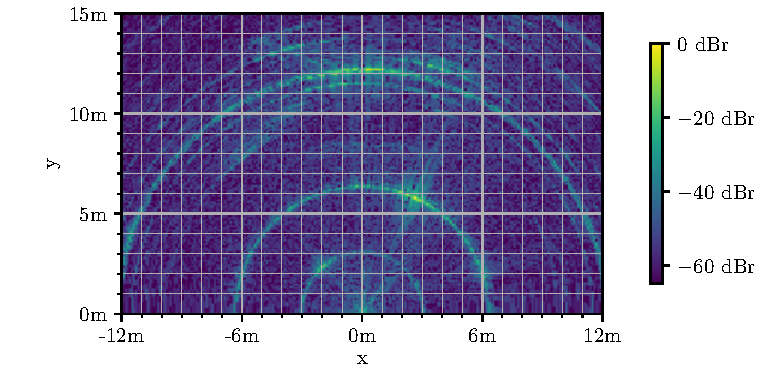
\includegraphics[width=\textwidth]{../figures/testimg_uncalibrated_fft.pdf}
        \subcaption{uncalibrated}
    \end{subfigure}
    \begin{subfigure}{0.8\textwidth}
        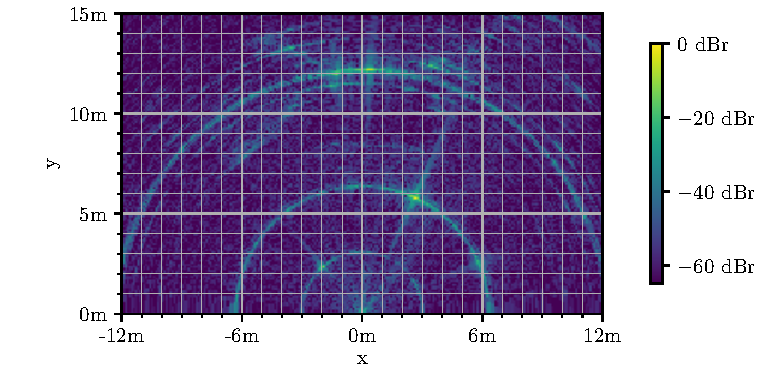
\includegraphics[width=\textwidth]{../figures/testimg_calibrated_fft.pdf}
        \subcaption{calibrated}
    \end{subfigure}
    \caption{FFT-based image generated from real data}
    \label{fig:fft_testimg}
\end{figure}
Calibration increases output SNR: less noise visible around [0m,7m]. Also reduces peak width in azimuth. Tower outline easier to make out.
Still fairly broad peaks, esp. in azimuth. CF azimuth theoretical peak: -40dB SLL. Clearer images: decrease dynamic range.

TO DO:

- image for approximate ground truth

- maybe 3d image?

- Runtime, real-time capabilities


\section{Backprojection Imaging}

The second imaging algorithm to be implemented is backprojection.
A detailed description of the algorithm can be found in section \ref{ssec:bp_imaging_theory},
but the gist of it is the following:

Backprojection works by computing the correlation between the incoming time data
and the signal of an ideal point scatterer (see eqn. \ref{eqn:ideal_scatterer})
at an arbitrary set of locations. The signal uses the measured antenna gains at that location.
Assuming the antenna gains to be static,
the ideal signals can be pre-computed to be used to generate images for multiple measurements.
An example implementation in PyTorch is shown in code listing \ref{lst:bp_img}.

TODO:

- how to calculate BP weights from measured antenna gains
\\

A major limitation of the way the backprojection algorithm is currently implemented is its scalability.
Pre-calculating the weights, while allowing for decent opportunites in decreasing the runtime through parallel processing,
quickly use a prohibitive amount of memory.

If there are $Z$ individual locations, $M$ sample points in time and $K$ channels, then $M \cdot K \cdot Z$ weights need to be computed.
For example, the weights for a uniformly spaced image with a rather low resolution of  $Z = 100 \cdot 10 \cdot 100 =$ \SI{100}{kilovoxels},
at $K=192$ and $M=1022$, stored as complex numbers consisting of two \SI{64}{bit} floating point numbers, would require
\begin{align*}
      & M \cdot K \cdot Z \cdot 2 \cdot \SI{64}{\bit} \\
    = & 1022 \cdot 192 \cdot 10^5 \cdot \SI{16}{byte} \\
    = & \SI{3.14e12}{byte} = \SI{3.14}{\tera\byte}
\end{align*}
of memory.
With the projections of Moore's law [citation needed],
this amount of memory should be available in consumer-level computers by the year 2050.
Until then, the memory requirements has to be reduced by re-computing the weights
and applying them to the input data along an arbitrary dimension.
For example, recomputing them for every of the sampled time points would reduce
the memory requirements by a factor of 1022 to only around \SI{3}{\giga\byte}.


\begin{figure}[h]
    \centering
    \begin{subfigure}[t]{\textwidth}
        \centering
        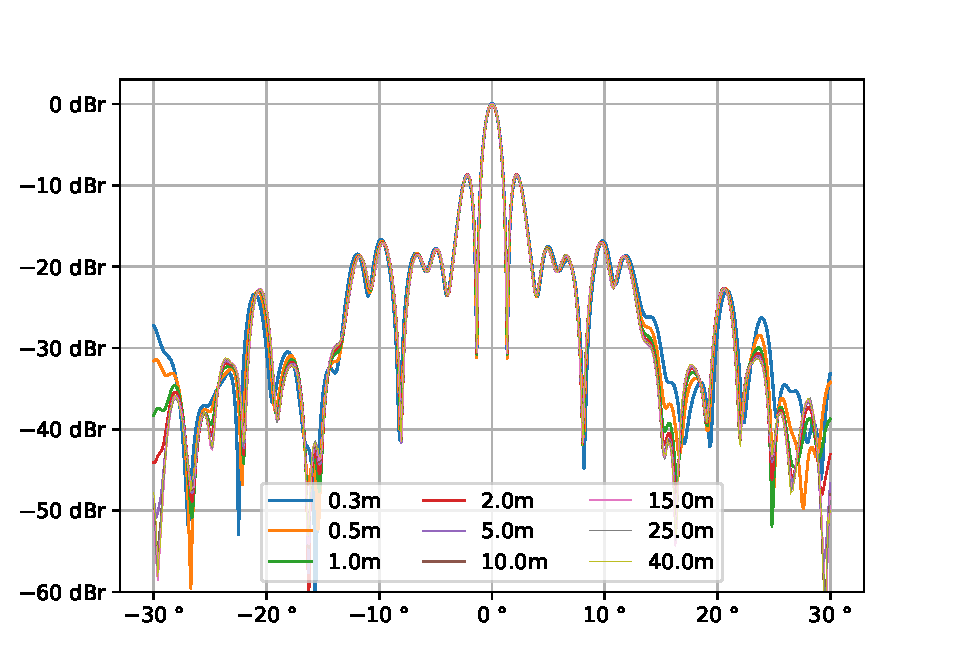
\includegraphics[width=\textwidth]{../figures/bp_azm_peak.pdf}
        \subcaption{azimuth}
        \label{fig:bp_azm_peak}
    \end{subfigure}

    \begin{subfigure}[position]{\textwidth}
        \centering
        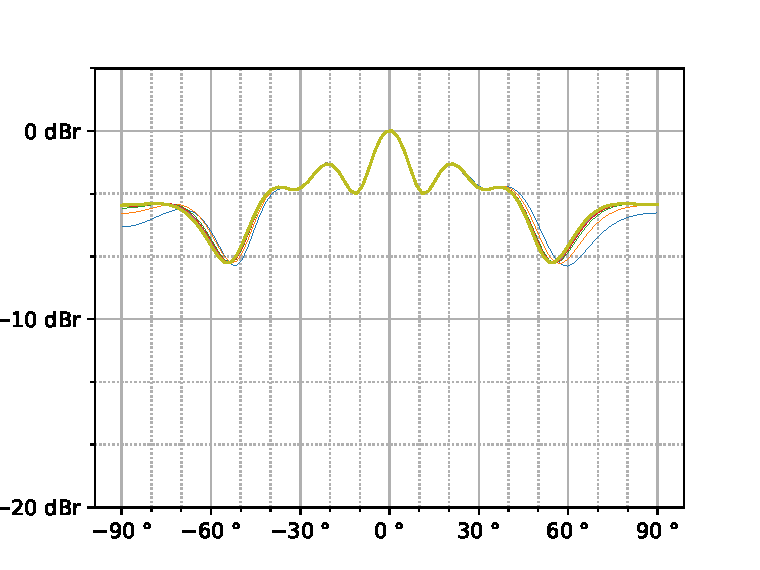
\includegraphics[width=0.8\textwidth]{../figures/bp_elv_peak.pdf}
        \subcaption{elevation}
        \label{fig:bp_elv_peak}
    \end{subfigure}

    \caption{iMCR backprojection direction of arrival estimation: theoretical accuracy for an ideal point scatterer at different ranges}
\end{figure}
\subsection{Direction of Arrival Accuracy}

To better understand the DoA-estimation capabilities of the algorithm,
the azimuth and elevation is simulated for multiple distances to illustrate the impact of near-field conditions.
The same input signal as in section \ref{ssec:fft_doa} is used.
\\

The image is computed for multiple distances at resolution
$N_{range} = 1$, ${N_{azimuth} = 512}$ and $N_{elevation} = 1$.
Naturally, the range of the image is set to the range of the ideal target each time.
The resulting peaks in azimuth and elevation are shown in figures \ref{fig:bp_azm_peak} and \ref{fig:bp_elv_peak}, respectively.


In both azimuth and elevation, it can be seen that the peak no longer deteriorates in near-field conditions.
The peak and most side lobes remain virtually identical across all considered ranges.
In azimuth, the level of the sidelobes stabilizes at around \SIrange{30}{40}{\dB} below the peak,
while in elevation, the sidelobe level is merely \SIrange{3}{6}{\dB} below the peak.

In azimuth, the half-power beamwidth is approximately $\theta_{\SI{3}{\dB}}=$ \SI{1.6}{\degree} and
the quarter-power beamwidth approximately $\theta_{\SI{6}{\dB}}=$ \SI{2.4}{\degree}.
In elevation, the half-power beamwidth is approximately $\phi_{\SI{3}{\dB}}=$ \SI{20}{\degree} and
the quarter-power beamwidth approximately $\phi_{\SI{6}{\dB}}=$ \SI{100}{\degree}.

TODO:

- discuss windowing

- discuss elevation/azimuth trade-off: should elevation-channels contribute more?


\newpage
\subsection{Test Image}
The theoretical capabilities of the backprojection algorithm are again tested for real world applications,
using the same scene as in section \ref{ssec:fft_result}.

Once again, the target 2D image spans a $24 \times$\SI{15}{\m} area in the horizontal plane,
with square pixels of edge length \SI{10}{\cm},
and the sensor located on one of the image's long sides, namely $[x,y] = [0,0]$m.
Unlike the FFT-based approach,
the backprojection algorithm allows for an arbitrary set of sample points,
so no further transformations are required.\\
\begin{figure}[t]
    \centering
    \begin{subfigure}[t]{0.8\textwidth}
        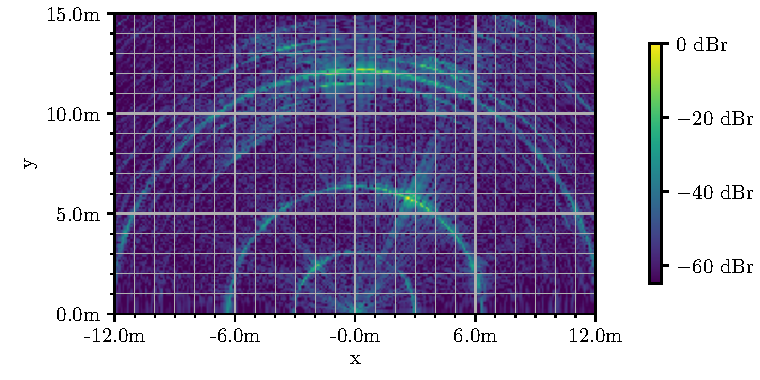
\includegraphics[width=\textwidth]{../figures/testimg_uncalibrated_bp.pdf}
        \subcaption{uncalibrated}
    \end{subfigure}
    \begin{subfigure}[t]{0.8\textwidth}
        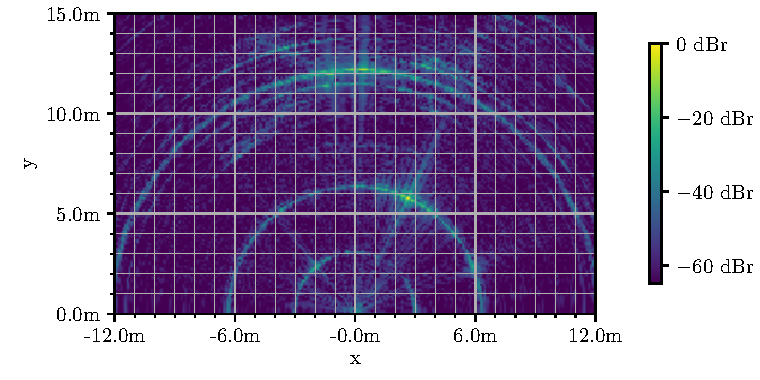
\includegraphics[width=\textwidth]{../figures/testimg_calibrated_bp.pdf}
        \subcaption{calibrated}
    \end{subfigure}
    \caption{Backprojection image generated from real data}
    \label{fig:bp_testimg}
\end{figure}
Figure \ref{fig:bp_testimg} shows the resulting image with and without calibration.
Calibration increases output SNR: less noise visible around [0m,7m].
Also reduces peak width in azimuth. Tower outline easier to make out.
Still fairly broad peaks, esp. in azimuth.
CF azimuth theoretical peak: -40dB SLL. Clearer images: decrease dynamic range.


- improve antenna gain model

- use locational calibration for test image

\section{Hybrid Approach}

Compared to the FFT-based approach, the backprojection algorithm is a lot more computationally intensive,
taking multiple orders of magnitude longer to compute a single 2D image.

    [maybe: talk about $\mathcal O(MlogN) \ll \mathcal O(MN)$]

As explained in section \ref{ssec:bp_imaging_theory},
it is possible to replace part of the computation with an FFT,
taking advantage of the increased speed and lower memory consumption of the FFT-algorithm,
while sacrificing some accuracy.

An example implementation of the backprojection-FFT-hybrid algorithm can be found in \ref{lst:hybrid_img}.
Its theoretical performance is investigated in the next section. Afterwards, a test image is computed.
\subsection{Direction of Arrival Accuracy}

- Discuss Phase error due to frequency quantization

- Plot: near-field beampattern for different FFT-lengths

\begin{figure}[h]
    \centering
    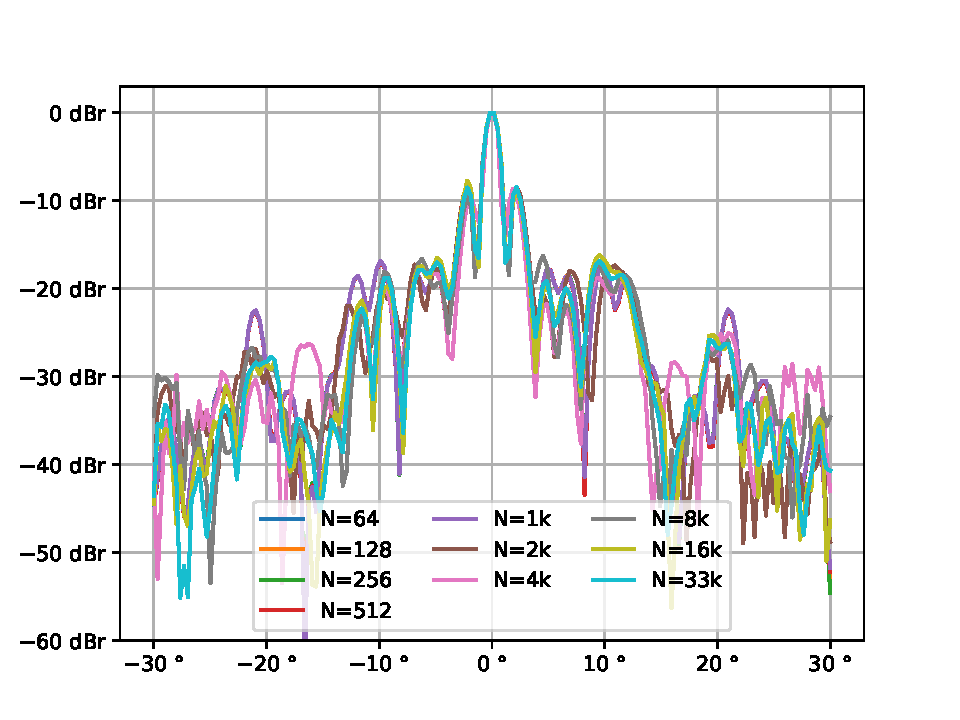
\includegraphics[width=\textwidth]{../figures/hybrid_azm_peak.pdf}
    \caption{iMCR Backprojection-FFT-Hybrid direction of arrival estimation: theoretical accuracy in azimuth for an ideal point scatterer at spectral resolutions}
    \label{fig:hybrid_azm_peak}
\end{figure}

\subsection{Test Image}

\section{Conclusion}


% 28.2.: theory
% 29.2.: stability
% 1.3.: antennas
% 2.3.: imaging
% 3.3.: Conclusion and discussion
% 4.3.: formatting, printing
\chapter{Conclusions}

\appendix
\printbibliography[heading=bibnumbered]
\chapter{Code}
\section{Introduction to PyTorch Sensor Processing}
\label{app:pytorch_tutorial}
Pytorch is a machine learning framework that provides Tensor processing.
A brief introduction of some of is features is provided here,
the full documentation is available online \cite{pytorch}.
Pytorch Tensors can be created from python lists,
or with a utility function like \verb|zeros()|, \verb|ones()| or \verb|full()|:
\lstset{
    language = Python ,
    columns = flexible ,
    escapeinside = {<@}{@>} ,
    frame = lines ,
    alsoletter = > ,
    morekeywords = {>>>} ,
    style=mystyle
}
\begin{lstlisting}
>>> import torch
>>> torch.tensor(list(range(2)))
tensor([0, 1])
>>> torch.ones((2,3))
tensor([[1., 1., 1.],
        [1., 1., 1.]])
\end{lstlisting}

Python's basic binary operators, such as \verb|+,-,*| or \verb|/|, can be used to operate on tensors.
If both tensors are the same size, the operation is done element by element, similar to the hadamard product of matrices.
Scalars can also be applied to tensors.
\begin{lstlisting}
>>> torch.tensor(list(range(2))) + torch.ones(2)
tensor([1., 2.])
>>> 5 + torch.zeros(2)
tensor([5.,5.])
\end{lstlisting}

These operations are also allowed for tensors of different size, if their shapes follow the requirement that
``[...] iterating over the dimension sizes, starting at the trailing dimension,
the dimension sizes must either be equal, one of them is 1, or one of them does not exist.''\footnote{
    see \url{https://pytorch.org/docs/stable/notes/broadcasting.html}
}\newpage

For example, a $3 \times 2\times 1$ tensor and a $1 \times 2$ tensor are broadcastable:
\begin{lstlisting}
>>> a = torch.tensor([[[0],[1]],[[2],[3]],[[4],[5]]])
>>> b = torch.tensor([[1,10]])
>>> a.shape, b.shape
(torch.Size([3, 2, 1]), torch.Size([1, 2]))
>>> a+b
tensor([[[ 1, 10],
         [ 2, 11]],

        [[ 3, 12],
         [ 4, 13]],

        [[ 5, 14],
         [ 6, 15]]])
\end{lstlisting}
In the third dimension, the elements of tensor \verb|a| are broadcast onto the elements of tensor \verb|b|.
In the second dimension, the inverse is the case. The resulting tensor has the shape $3 \times 2\times 2$.

Tensor indexing of one-dimensional tensors is identical to list indexing in python;
and multi-dimensional tensors are indexed with a tuple of indices or slices.
For example, to select all first elements of the previous result's third dimension, the following syntax is used:
\begin{lstlisting}
>>> c=a+b
>>> c[:,:,0]
tensor([[1, 2],
        [3, 4],
        [5, 6]])
\end{lstlisting}
Dimensions where a single index was used are omitted from the result.
It is also possible to insert dimensions with the keyword \verb|None|:
\begin{lstlisting}
>>> c[:,:,0].shape
torch.Size([3, 2])
>>> c[:,None,:,0].shape
torch.Size([3, 1, 2])
\end{lstlisting}

Besides these basic operations, a plethora of functions is already implemented for tensors.
Often, for each function operating on a tensor,
there is also an equivalent member function of the class tensor that does the same.
This makes composing functions a lot easier, because no nested parentheses are required:
\begin{lstlisting}
>>> a = torch.randn((1,100))
>>> 20*torch.log10(torch.abs(torch.mean(a)))
tensor(-16.3953)
>>> 20*a.mean().abs().log10()
tensor(-16.3953)
\end{lstlisting}

\newpage
\section{Listings}
\lstinputlisting[
    caption={PyTorch implementation of the FFT-based imaging algorithm},
    language=Python,
    firstline=3,
    float,
    floatplacement=ht,
    label=lst:fft_img]{../figures/scripts/3.1_imaging/fft_example_impl.py}

\lstinputlisting[
    caption={PyTorch implementation of the backprojection imaging algorithm},
    language=Python,
    firstline=3,
    lastline=24,
    float,
    floatplacement=ht,
    label=lst:bp_img]{../figures/scripts/3.1_imaging/bp_example_impl.py}
\lstinputlisting[
    caption={PyTorch computation of the channel-wise time of flight for a given position},
    language=Python,
    firstline=26,
    lastline=40,
    float,
    floatplacement=ht,
    label=lst:bp_tof]{../figures/scripts/3.1_imaging/bp_example_impl.py}
\lstinputlisting[
    caption={PyTorch computation of uniformly spaced sample positions in different coordinate systems},
    language=Python,
    firstline=42,
    float,
    floatplacement=ht,
    label=lst:bp_pos]{../figures/scripts/3.1_imaging/bp_example_impl.py}

\lstinputlisting[
    caption={PyTorch implementation of the FFT-backprojection hybrid algorithm},
    language=Python,
    firstline=4,
    lastline=30,
    float,
    floatplacement=ht,
    label=lst:hybrid_img]{../figures/scripts/3.1_imaging/hybrid_example_impl.py}

\listoffigures
\listoftables
\end{document}